\documentclass[11pt,a4paper]{article}
\usepackage{fontspec}
\setmainfont{Noto Serif}
\setsansfont{Noto Sans}
\setmonofont{Noto Sans Mono}[Scale=0.86]
% fontspec handles Vietnamese Unicode; no external babel language package.
\usepackage{amsmath,amssymb,amsthm,mathtools}
\usepackage{geometry,booktabs,longtable,tabularx,array}
\usepackage{tikz}
\usetikzlibrary{arrows.meta,positioning,calc}
\usepackage{xcolor,hyperref,xurl,fancyhdr,enumitem}
\geometry{margin=2.2cm,headheight=15pt}
\definecolor{ink}{HTML}{183449}
\definecolor{teal}{HTML}{187C80}
\hypersetup{colorlinks=true,linkcolor=ink,citecolor=teal,urlcolor=teal,
pdftitle={ECDR: Giải thích toàn bộ nền tảng toán học},pdfauthor={ECDR Research}}
\urlstyle{same}
\setlength{\parindent}{0pt}
\setlength{\parskip}{5pt}
\setlength{\emergencystretch}{3em}
\setlength{\tabcolsep}{4pt}
\renewcommand{\arraystretch}{1.16}
\setlist{nosep,leftmargin=1.5em}
\newcolumntype{Y}{>{\raggedright\arraybackslash}X}
\newcommand{\R}{\mathbb R}
\newcommand{\norm}[1]{\left\lVert#1\right\rVert}
\newcommand{\abs}[1]{\left\lvert#1\right\rvert}
\newcommand{\code}[1]{{\small\ttfamily\nolinkurl{#1}}}
\newcommand{\relu}{\operatorname{ReLU}}
\newcommand{\diag}{\operatorname{diag}}
\newcommand{\vecop}{\operatorname{vec}}
\newcommand{\ind}{\mathbf1}
\newcommand{\E}{\mathbb E}
\newcommand{\Sset}{\mathcal S}
\newcommand{\Uset}{\mathcal U}
\newtheorem{proposition}{Mệnh đề}[section]
\newtheorem{theorem}[proposition]{Định lý}
\newtheorem{lemma}[proposition]{Bổ đề}
\theoremstyle{definition}
\newtheorem{example}[proposition]{Ví dụ}
\renewcommand{\proofname}{Chứng minh}
\renewcommand{\contentsname}{Mục lục}
\renewcommand{\tablename}{Bảng}
\renewcommand{\figurename}{Hình}
\renewcommand{\refname}{Tài liệu tham khảo}
\pagestyle{fancy}
\fancyhf{}
\fancyhead[L]{\small\textcolor{ink}{ECDR | Giải thích toán học}}
\fancyhead[R]{\small Tài liệu đồng hành Week 1--3}
\fancyfoot[L]{\small 03/11/2026}
\fancyfoot[R]{\thepage}
\begin{document}
\hypersetup{pageanchor=false}
\begin{titlepage}
\vspace*{1.1cm}
{\Large\color{teal} TÀI LIỆU GIẢI THÍCH CHI TIẾT\par}
\vspace{0.6cm}
{\huge\bfseries\color{ink} Toàn bộ nền tảng\\toán học của ECDR\par}
\vspace{0.7cm}
{\Large Từ dữ liệu cảm biến đến chứng nhận quyết định,\\
reuse nhiều bước và điều kiện hòa vốn\par}
\vspace{1cm}
\begin{tabularx}{\linewidth}{@{}p{3cm}Y@{}}\toprule
Vai trò & Tài liệu đồng hành với báo cáo lý thuyết Week 1--3.\\
Cách giải thích & Ký hiệu $\to$ trực giác $\to$ từng bước suy ra $\to$
ví dụ số $\to$ điều kiện và giới hạn.\\
Phạm vi & Bao gồm phần toán của data, CNN, probability, certification,
structured domains, lifecycle và cost; không chỉ Lipschitz.\\
Ví dụ xuyên suốt & Một CNN nhỏ tính tay được; mọi số trong ví dụ là minh
họa toán học, không phải mô hình HAPT đã train.\\
Nguồn đối chiếu & \code{03_Week_3_Mathematical_Foundations.tex}, frozen Week1--2 và các nguồn gốc trong bibliography.\\\bottomrule
\end{tabularx}
\vfill
\textbf{Mục tiêu đọc.} Sau khi đọc, người đọc có thể giải thích mỗi công
thức đang tính đại lượng gì, vì sao bất đẳng thức có chiều đó, cần giả thiết
nào và điều gì vẫn chưa được kết luận. Số học dùng số thực, trừ mục riêng
về sai số chương trình. Tài liệu này bổ sung diễn giải; không tuyên bố các
kết quả nền tảng là định lý mới của ECDR.
\end{titlepage}
\hypersetup{pageanchor=true}
\pagenumbering{arabic}

\section*{Lộ trình đọc}
\addcontentsline{toc}{section}{Lộ trình đọc}
ECDR muốn trả một quyết định đã biết khi có bằng chứng rằng quyết định đó
vẫn đúng với reference hiện tại. Chuỗi lập luận cần đủ sáu cầu nối:
\begin{equation*}
\text{data}\to\text{input space}\to\text{domain}\to\text{margin bound}
\to\text{membership và reuse}\to\text{total cost}.
\end{equation*}
Thiếu một cầu nối, ta dễ nhầm ``hai cửa sổ giống nhau'' với ``CNN chắc chắn
cùng quyết định'', hoặc nhầm ``tránh được CNN'' với ``hệ thống nhanh hơn''.

Đọc mục 1--7 để hiểu data và classifier; mục 8--16 để hiểu proof và miền;
mục 17--21 để thấy CNN/window/membership/lifecycle nối với nhau; mục
22--24 để hiểu numerical semantics, cost và evidence. Các phụ lục map đủ
các nhóm công thức và H01--H24 của báo cáo chính.

Một số tên ký hiệu được làm rõ để tránh overload: $d_x=CW$ là input
dimension; $d_h$ là số feature channels trước head; $n$ là số feature
positions; $Q$ là horizon theo số bước, không phải feature tensor $H(X)$;
$\rho_b$ là build/query, không phải bias hay box budget.

\begingroup
\small
\setlength{\parskip}{0pt}
\tableofcontents
\endgroup
\clearpage

\section*{Đọc cùng actual reference K=12}
\addcontentsline{toc}{section}{Đọc cùng actual reference K=12}
Tài liệu này giải thích vì sao công thức cần thiết và cách thay số; báo cáo
A giữ chứng minh đầy đủ và ledger audit. Hai vai trò khác nhau.
Reference hiện tại là \code{SmallCNN1D(num_classes=12)} tại commit xuất phát
\code{8d4ebae576e612837dfd2f3cdcbaab737a705c4b}, không phải toy valid--GAP.

\textbf{Phân biệt bốn số.} $C=6$ là số channel cảm biến, $W=128$ là số
sample trong một window, $s=64$ là số sample dịch, $K=12$ là số activity
logits. Input có $CW=768$ scalar; new wave có $Cs=384$ scalar; mỗi winner
phải so với $K-1=11$ competitors. Tăng K không tăng số channel cảm biến.

\textbf{Từ raw đến reference.} $X\in\R^{6\times128}$ chứa gia tốc theo$g$
và vận tốc góc theo rad/s. $\mu,\sigma\in\R^6$ là constants train-fit đã
khóa. $Z=N(X)=(X-\mu)/\sigma$ là tensor normalized không có đơn vị;
$f_\theta(Z)$ có 12 logits, $F(X)=f_\theta(N(X))$ là ideal real map.
$\widehat F(X)$ là executable float32; proof của $F$ cần numerical bridge
mới áp được cho $\widehat F$. Lưu constants float32 chính xác xác định một
hàm toán học; nó không tự bao sai số của các phép tính float32 sau đó.

\begin{table}[!htbp]\centering\small
\caption{Kích thước actual graph, đọc theo một query $B=1$.}
\begin{tabularx}{\linewidth}{@{}p{7.2cm}Y@{}}\toprule
Bước & Tensor output\\\midrule
Input; Conv6$\to$32 k5 p2; BN--ReLU & $1\times32\times128$ sau Conv/BN/ReLU\\
Pool2; Conv32$\to$64 k3 p1; BN--ReLU & $1\times64\times64$ sau Conv thứ hai\\
Pool2; Conv64$\to$64 k3 p1; BN--ReLU & $1\times64\times32$\\
Flatten; Linear2048$\to$128; ReLU & $1\times128$ sau Linear/ReLU\\
Linear128$\to$12 & $1\times12$ logits\\\bottomrule
\end{tabularx}
\end{table}
Checkpoint ở \code{output/week1_closeout_20261102/reference/selected_best.pt},
SHA-256 \code{8ffc5dd8eb0e9cdf832160d074f3ae816ae6cba02adf7214a63a8b623303adb1}.
Preprocessing ID \code{aa8e1cc20829307187e0a78200f9957f7dd068b1dc26063c2720ad832bb2fd6e}.
283,692 trainable parameters; BN running buffers cũng thuộc identity nhưng
không tính như trainable parameters. Full test stream 5,053 và supervised
subset 3,572 có mẫu số khác nhau. Accuracy 0.8905375 và macro-F1 0.7762645
chỉ thuộc subset có nhãn; G2 giữ HOLD.

\subsection*{Ví dụ1: point margin, regional minimum và lower bound}
Đây là ví dụ hai lớp, không phải output của checkpoint. Cho
$F_1(x)=1-x,F_2(x)=0$, anchor$x^r=0$, winner$c=1$ và miền$[-0.2,0.2]$.
Point margin là$g_{12}(0)=1$. Exact regional minimum là
$\inf_{x\in[-0.2,0.2]}(1-x)=0.8$. Một thuật toán có thể chỉ trả lower
bound$\ell=0.7$: vì$0.7\le0.8$ và$0.7>0$, vẫn chứng nhận được miền.
Nếu nó trả$-0.1$, không có certificate từ bound đó, dù exact minimum vẫn
$0.8$. Nếu đổi miền thành$[-2,2]$, point margin vẫn1 nhưng minimum$-1$.
Với actual model phải thực hiện cùng lập luận cho đủ 11 margins, không chỉ
logit đứng thứ hai tại anchor vì competitor mạnh nhất có thể đổi trong miền.

\subsection*{Ví dụ2: BN, MaxPool và direct margin, tính từng bước}
Các constants nhỏ sau chỉ dùng minh họa operator của actual graph.
BN eval có dạng $y=a v+b$ với
$a=\gamma/\sqrt{\mathrm{running\_var}+\epsilon_{\rm BN}}$,
$b=\beta-a\,\mathrm{running\_mean}$. Nếu$v\in[-1,2]$, $a=-2,b=1$,
thì $y\in[-2\cdot2+1,-2\cdot(-1)+1]=[-3,3]$; scale âm đòi đổi đầu mút.
ReLU cho interval$[0,3]$. Pool của hai pre-pool intervals$[0,3]$ và$[2,4]$
được bao bởi$[\max(0,2),\max(3,4)]=[2,4]$. Nó không affine khi winning
pool index thay đổi, dù từng nhánh là một phép chọn tọa độ.

Xét hidden interval$h_1,h_2\in[0,2]$, final rows$W_c=(2,1)$,
$W_j=(1,1)$ và biases$b_c=1,b_j=0$. Bound riêng logits là
$F_c\in[1,7]$, $F_j\in[0,4]$ nên lower margin$1-4=-3$.
Gộp rows trước: $g_{cj}=(W_c-W_j)h+1=h_1+1\in[1,3]$,
lower margin1. Term$h_2$ đã triệt tiêu. Đây là lý do bound direct margin,
không chứng minh direct margin đủ chặt ở mọi lớp phi tuyến.

Một phản ví dụ cho IBP nói chung: $h_1=h_2=\relu(x+1)$,
$x\in[-1,1]$, $g=1+h_1-h_2$. True margin luôn 1; nếu hai hidden units bị interval hóa độc lập
thành$[0,2]^2$, direct-margin IBP trả$1+0-2=-1$ và không nhận strict certificate.
Việc gộp final rows có thể sửa một số cancellation, nhưng không khôi phục
mọi dependency đã mất ở tầng trước. Đây là incompleteness, không unsoundness.

\subsection*{Ví dụ3: suy ra12 aligned feature positions của actual graph}
Dùng index zero-based. Conv1 tại$i$ nhìn$[i-2,i+2]$.
Pool1 tại$i$ lấy hai Conv1 positions$2i,2i+1$, nên nhìn
$[2i-2,2i+3]$. Conv2 dùng$i-1,i,i+1$ của Pool1, nên nhìn
$[2i-4,2i+5]$. Pool2 cho$[4i-4,4i+7]$; Conv3 cho
\[
 [4j-8,4j+11],\qquad (4j+11)-(4j-8)+1=20.
\]
Jump4 nghĩa là sang feature tiếp theo dịch4 raw samples. Dịch64 samples
là dịch$64/4=16$ final features. Để RF nằm trong shared half$[0,63]$:
\[
 4j-8\ge0\Rightarrow j\ge2,\qquad
 4j+11\le63\Rightarrow j\le13.
\]
Vì vậy $H_j(X_{t+1})=H_{j+16}(X_t)$ cho$j=2,\ldots,13$ với same
pool phase, BN eval frozen và time-homogeneous normalization. Có
$13-2+1=12$ positions, mỗi vị trí64 channels:768 feature scalars.
Tại$j=2$, RF$[0,19]$ chuyển sang$[64,83]$ ở window cũ.
Tại$j=13$, RF$[44,63]$ chuyển sang$[108,127]$.
$j=1$ dùng padding mới; $j=14$ dùng new wave nên không được theorem bảo đảm.
Interval$[4j-9,4j+10]$ đôi khi được nhắc có đúng width20 nhưng sai origin.

\textbf{Vì sao equality này chưa cho reuse class?} Actual Flatten sắp
$(channel,time)$ vào 2048 coordinates. Một dense head nhỏ có thể đặt weight1
ở position2 và weight0 ở position18. Dù new feature2 bằng old feature18,
hai output vẫn dùng coefficients khác nhau. Actual head còn có ReLU của
128 hidden units. Vì vậy không thể thế công thức GAP vào head này.
Các tính toán valid--GAP ở những mục sau vẫn được giữ để hiểu định lý H13
cũ và H14; chúng là alternative/historical architecture với giả thiết riêng.

\subsection*{Ví dụ4: fixed-overlap box và kiểm biên bảo thủ}
Với một channel toy$W=4,s=2$, anchor normalized$(1,2,3,4)$ thì next
window có dạng$(3,4,u_1,u_2)$. Nếu$u_1\in[4.9,5.1]$,
$u_2\in[5.8,6.2]$, chỉ hai biến tự do. Query$(3,4,5,6)$ thuộc miền;
query$(3.01,4,5,6)$ không thuộc dù tail đúng. Không có trusted prefix state
thì không được bỏ kiểm hai tọa độ đầu. Trong HAPT, ví dụ này tăng lên 384
prefix scalars và 384 tail scalars. K=12 không tác động các số này.

Nếu normalization của raw query chỉ được biết nằm trong interval
$[\underline z_i,\overline z_i]$, muốn accept phải chứng minh cả interval
nằm trong certified interval$[L_i,U_i]$. Điều kiện là
$\underline z_i\ge L_i$ và$\overline z_i\le U_i$.
Ví dụ certified$[0,1]$, enclosure$[0.999,1.001]$ phải reject dù midpoint1.
Sai số mỗi operator và mỗi bước tính bound cần có biện minh; cộng tùy ý
$10^{-6}$ hoặc chỉ ép float64 không phải proof cho float32.

\subsection*{Ví dụ5: no-hit và chi phí âm là kết quả hợp lệ}
Giả sử có$N=100$ query, không query nào được reuse và mọi query fallback
đúng reference. All-query agreement có thể100/100, nhưng
$A_{\rm reuse}=0/0$ là N/A; $r_{\rm cert}=0/100=0$.
Trong mô hình giả định$t_f=0.2$ms, $t_v+t_m=0.01$ms,
$B=10$ builds, $t_b=2$ms, mean ECDR cost là
$0.01+0.2+(10/100)\cdot2=0.41$ms, speed ratio$0.2/0.41=0.488$.
Đây là thay số toy, không phải benchmark. Nó giải thích H19--H20:
sound gate có thể hữu ích về correctness nhưng không tạo saving.

\section{Đọc ngôn ngữ toán học trong báo cáo}
\subsection{Điểm, tập, hàm và lượng từ}
Một điểm $x\in\R^{d_x}$ là \emph{một đầu vào cụ thể}. Một tập
$\Sset\subseteq\R^{d_x}$ là \emph{nhiều đầu vào có thể xét}. Hàm
$F:\R^{d_x}\to\R^K$ nhận một điểm và trả $K$ số. Khi viết
\begin{equation}
\forall x\in\Sset,\quad h(x)=c,
\label{eq:universal}
\end{equation}
ta nói ``với mọi điểm trong miền này, reference đều chọn lớp $c$''. Nó
mạnh hơn việc kiểm một vài điểm. Viết $\exists x\in\Sset:h(x)\ne c$ chỉ cần
một điểm phản ví dụ để bác (\ref{eq:universal}).

Ký hiệu $A\Rightarrow B$ nói $A$ là điều kiện đủ cho $B$; $B$ là điều kiện
cần của $A$. Ký hiệu $A\Leftrightarrow B$ đòi cả hai chiều. Một thuật toán
có thể không nhận được certificate dù $B$ thực sự đúng; vì vậy không được
đổi mọi dấu $\Rightarrow$ thành $\Leftrightarrow$.

\subsection{Tích vô hướng, ma trận, các norm và đơn vị}
Với $a,x\in\R^m$, $a^\top x=\sum_{i=1}^m a_ix_i$ là tích vô hướng.
Nếu $A\in\R^{K\times m}$ thì $Ax$ có $K$ phần tử, mỗi row của $A$ tạo một
tích vô hướng. $A^\top$ chuyển row thành column; ký hiệu này không phải
nghịch đảo.

Ba norm thường dùng là
\begin{equation}
\norm{v}_1=\sum_i|v_i|,\qquad
\norm{v}_2=\sqrt{\sum_i v_i^2},\qquad
\norm{v}_\infty=\max_i|v_i|.
\end{equation}
Với $v=(3,-4)$, các giá trị lần lượt là $7,5,4$. Ball $L_2$ ở 2D là hình
tròn; ball $L_\infty$ là hình vuông; ball $L_1$ là hình thoi. Tất cả đều
có tâm và bán kính, nhưng mỗi norm định nghĩa ``gần'' khác nhau.

\begin{figure}[!htbp]\centering
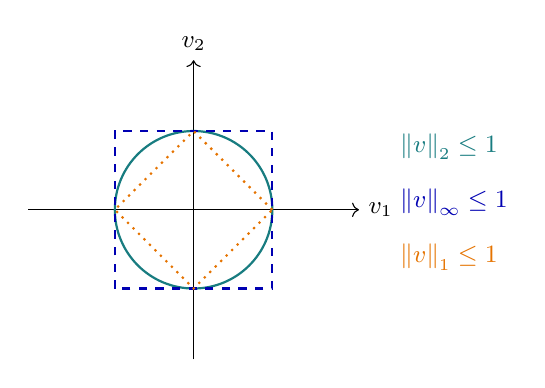
\begin{tikzpicture}[scale=1.0,font=\small]
\draw[->] (-2.1,0)--(2.1,0) node[right]{$v_1$};
\draw[->] (0,-1.9)--(0,1.9) node[above]{$v_2$};
\draw[teal,thick] (0,0) circle (1);
\draw[blue!70!black,dashed,thick] (-1,-1) rectangle (1,1);
\draw[orange!90!black,dotted,thick] (1,0)--(0,1)--(-1,0)--(0,-1)--cycle;
\node[anchor=west,teal] at (2.5,0.8){$\norm{v}_2\le1$};
\node[anchor=west,blue!70!black] at (2.5,0.1){$\norm{v}_\infty\le1$};
\node[anchor=west,orange!90!black] at (2.5,-0.6){$\norm{v}_1\le1$};
\end{tikzpicture}
\caption{Hình học minh họa của ba unit balls; cùng radius không có nghĩa
cùng tập. Hình dùng tọa độ toán học không có sensor units.}
\end{figure}

Với ma trận $X$, Frobenius norm là
$\norm{X}_F=\sqrt{\sum_{c,i}X_{ci}^2}$. Nó bằng Euclidean norm của vector
chứa cùng các giá trị. Norm của raw acceleration và raw angular velocity
cần quy ước scale: không nên coi một đơn vị $g$ và một đơn vị rad/s là
những biến thiên vật lý tương đương chỉ vì hai số cùng bằng 1.

\section{Dữ liệu được biến thành một điểm toán học như thế nào?}
\subsection{Từ sample đến recording và window}
Theo mô tả HAPT \cite{hapt}, một sample gồm ba trục gia tốc và ba trục vận
tốc góc. Đặt
\begin{equation}
s[n]=(a_x[n],a_y[n],a_z[n],\omega_x[n],\omega_y[n],\omega_z[n])^\top.
\end{equation}
Ở đây $n$ đếm sample, không phải giây; timestamp tương ứng là $n/f_s$ với
$f_s=50$ sample/s. Một recording có $T$ sample được xếp thành ma trận
$S\in\R^{6\times T}$, mỗi column là một sample. Đây là nhánh raw inertial
data; vector 561 features được dựng sẵn trong một nhánh HAPT khác không
phải input tensor đang xét. Raw acceleration dùng đơn vị $g$ và angular
velocity dùng rad/s theo README; normalization không tự tách gravity hay
sửa calibration của sensor.

Window thứ $t$ lấy $W$ column bắt đầu ở $ts$:
\begin{equation}
X_t[:,i]=s[ts+i],\quad i=0,\ldots,W-1.
\label{eq:window}
\end{equation}
Dấu ``:'' lấy toàn bộ kênh; đoạn $[a:b]$ là half-open, chứa $a$ nhưng không
chứa $b$. Stride $s$ là số sample tiến thêm mỗi window. Với $C=6,W=128,s=64$,
\begin{align}
d_x=CW&=768, & W/f_s&=2.56\ \mathrm{s},\\
s/f_s&=1.28\ \mathrm{s}, & f_s/s&=0.78125\ \text{window/s}.
\end{align}
Window convention dùng $W/f_s$; thời gian từ sample đầu đến sample cuối là
$(W-1)/f_s=2.54$ s vì có 127 khoảng giữa 128 sample. Hai con số không mâu
thuẫn; chúng đếm hai đối tượng khác nhau.

\subsection{Vector hóa và kiểm dimension}
Đặt $x_{cW+i}=X[c,i]$ theo channel-major order. Với $C=2,W=3$,
\begin{equation}
X=\begin{pmatrix}1&2&3\\4&5&6\end{pmatrix}
\quad\longleftrightarrow\quad x=(1,2,3,4,5,6)^\top.
\end{equation}
Không mất số nào; chỉ đổi cách xếp. Nếu chọn time-major order thì vector
khác, nhưng có một permutation matrix $P$ đổi giữa hai vector. Do
$P^\top P=I$, $\norm{Px}_2^2=x^\top P^\top Px=x^\top x$.
Classifier và miền phải dùng cùng layout; bảo toàn norm không có nghĩa
được phép hoán vị input tùy ý rồi dùng nguyên weights CNN.

Một window float32 có $768\times4=3072$ byte, tức 3 KiB; new wave có
$6\times64\times4=1536$ byte. Đây chỉ là payload tensor, không phải RAM
toàn hệ thống, decoded dataset size hay GPU memory.

\section{Đếm window và gán nhãn: vì sao công thức có floor và ceil?}
\subsection{Số window trên recording}
Window start ở $ts$ và phải kết thúc trước hoặc tại $T$:
\begin{equation}
ts+W\le T\quad\Rightarrow\quad t\le\frac{T-W}{s}.
\end{equation}
$t$ nguyên không âm nên $t=0,1,\ldots,\lfloor(T-W)/s\rfloor$.
Vì đếm cả 0, số window là
\begin{equation}
n_T=\max\left(0,1+\left\lfloor\frac{T-W}{s}\right\rfloor\right).
\end{equation}
Với $T=1000,W=128,s=64$, $(T-W)/s=13.625$, nên có $14$ window,
start cuối $13\times64=832$, kết thúc ở 960. Start tiếp theo 896 kết thúc
ở 1024 nên không hợp lệ. Không nối recording; tổng corpus là tổng các
$n_T$ của từng recording.

\subsection{Pure window nằm trong label span}
Với span $[a,b)$, một window nằm trọn khi
$a\le ts$ và $ts+W\le b$. Kết hợp với recording limits,
\begin{equation}
\left\lceil\frac{\max(a,0)}s\right\rceil
\le t\le
\left\lfloor\frac{\min(b-W,T-W)}s\right\rfloor.
\end{equation}
Số nguyên trong đoạn là cận trên trừ cận dưới cộng 1, rồi lấy max với 0.
Ví dụ span $[100,400)$ trong recording đủ dài, $W=128,s=64$, cho
$t_{\min}=\lceil100/64\rceil=2$,
$t_{\max}=\lfloor272/64\rfloor=4$. Có ba starts 128,192,256. Start 320
không hợp lệ vì window sẽ chạm 448 ngoài span.

Span ngắn hơn $W$ không chứa pure window. Nếu hai span cùng nhãn tiếp giáp,
cần xác định có hợp nhất hay không trước khi cộng các count. Annotation
one-based/inclusive phải được quy về convention này; chỉ viết công thức
đúng không tự xác minh file annotation gốc đã được chuyển đúng.

\subsection{Tỉ lệ annotation và ngưỡng majority}
Đặt $n_k$ là số sample có nhãn $k$ trong window và $n_0$ là số sample chưa
annotation. Ta có $\sum_{k=0}^{12}n_k=W$. Một pure window có $n_k=W$ cho
một lớp; unlabeled có $n_0=W$. Majority policy trong báo cáo dùng
\begin{equation}
\max_{k\ge1}\frac{n_k}{W}\ge0.6,
\end{equation}
với điều kiện không pure. Vì $n_k$ nguyên, $W=128$ cần ít nhất
$\lceil76.8\rceil=77$ sample. Nếu $n_k=70,n_0=58$, tỉ lệ trên annotated
samples là 100\% nhưng tỉ lệ whole-window chỉ $70/128=54.6875\%$; policy
không nhận majority. Denominator là một phần của định nghĩa, không phải
chi tiết tùy chọn.

Schema HAPT có 12 nhãn; số lớp $K$ của classifier được chọn riêng. Các
count pure của snapshot báo cáo là $10361$, trong đó basic-6 là $10017$,
nên transition pure là $344$, tỉ lệ $344/10361\approx3.3201\%$. Con số này
là đặc tính của window policy và corpus lưu, không phải xác suất hoạt động
của người dùng ngoài thực tế.

\section{Normalization biến đổi cả input, metric và domain}
\subsection{Tại sao trừ mean rồi chia scale?}
Với train-fit mean $\mu_i$ và $\sigma_i>0$ lặp theo kênh,
\begin{equation}
z_i=\frac{x_i-\mu_i}{\sigma_i},\qquad
z=D_\sigma^{-1}(x-\mu).
\label{eq:normalization}
\end{equation}
Mean chuyển gốc tọa độ; scale thay độ dài một đơn vị. Ví dụ một raw coordinate
có $\mu=2,\sigma=0.5$, raw value 2.1 trở thành $(2.1-2)/0.5=0.2$.
Một coordinate khác có $\sigma=2$ thì cùng raw delta 0.1 chỉ thành 0.05.
Do đó một isotropic box trong normalized coordinates thường là anisotropic
box trong raw coordinates.

Lấy hiệu hai query, mean triệt tiêu:
\begin{align}
z-z_r&=D_\sigma^{-1}(x-x_r),\\
\norm{z-z_r}_2^2&=\sum_i\frac{(x_i-x_{r,i})^2}{\sigma_i^2}.
\end{align}
Đây là một weighted raw metric. Không được đo distance ở raw space rồi
so với radius được chứng nhận trong normalized space mà không transform.

\subsection{Biến đổi budget và affine certificate}
Nếu $|x_i-x_{r,i}|\le b_i^{\rm raw}$ thì normalized budget là
$b_i=b_i^{\rm raw}/\sigma_i$; ngược lại $b_i^{\rm raw}=\sigma_i b_i$.
Trong ví dụ $\sigma=0.5$, raw budget 0.1 tương đương normalized budget 0.2.

Giả sử bound normalized là $g(z)\ge a_z^\top z+\beta_z$ trên miền hợp lệ.
Thay (\ref{eq:normalization}) vào,
\begin{align}
a_z^\top D_\sigma^{-1}(x-\mu)+\beta_z
&=(D_\sigma^{-\top}a_z)^\top x
+\beta_z-a_z^\top D_\sigma^{-1}\mu,\\
a_x&=D_\sigma^{-\top}a_z,\qquad
\beta_x=\beta_z-a_z^\top D_\sigma^{-1}\mu.
\end{align}
Ví dụ scalar $a_z=3,\beta_z=1,\mu=2,\sigma=0.5$ cho $a_x=6,\beta_x=-11$.
Tại raw 2.1, hai biểu thức cùng bằng 1.6. Biến đổi công thức chỉ đúng về
đại số; vẫn phải biết bound normalized hợp lệ trên ảnh của raw domain.

\section{Sliding window: bằng nhau sau căn chỉnh khác với gần nhau}
\subsection{Viết toán tử bằng ma trận nhỏ}
Đặt $S_sX=[X[:,s:W],0]$ và $J_sU=[0,U]$. Khi đó
\begin{equation}
X_{t+1}=\mathcal T_s(X_t,U_{t+1})=S_sX_t+J_sU_{t+1}.
\end{equation}
Với một kênh $W=4,s=2$,
\begin{equation}
S_s=\begin{pmatrix}0&0&1&0\\0&0&0&1\\0&0&0&0\\0&0&0&0\end{pmatrix},\quad
J_s=\begin{pmatrix}0&0\\0&0\\1&0\\0&1\end{pmatrix}.
\end{equation}
Nhân $S_s$ với $(a,b,c,d)^\top$ cho $(c,d,0,0)^\top$; thêm
$J_s(u,v)^\top$ cho $(c,d,u,v)^\top$. Với nhiều kênh, áp cùng phép dịch
cho từng row hoặc dùng block-diagonal operator trong vectorized space.

\subsection{Suy ra overlap identity từng chỉ số}
Từ (\ref{eq:window}),
\begin{align}
X_{t+1}[:,i]&=s[(t+1)s+i]\\
&=s[ts+(i+s)]=X_t[:,i+s],\quad i<W-s.
\end{align}
Hai biểu thức truy đúng một raw sample. Đó là lý do equality chính xác,
không phải vì người đang ``cùng hoạt động''. Với HAPT có $6(128-64)=384$
giá trị overlap và $6\times64=384$ giá trị mới.

Lấy hiệu ở cùng tọa độ cho
\begin{equation}
X_{t+1}-X_t=(S_s-I)X_t+J_sU_{t+1}.
\end{equation}
Hạng $(S_s-I)X_t$ có thể lớn. Ví dụ $(0,0,M,M)$ chuyển thành
$(M,M,0,0)$ với new wave 0, giữ 50\% overlap sau alignment nhưng distance
Euclidean là $\sqrt{4M^2}=2|M|$. Không có cận nhỏ độc lập với $M$.
Nếu thêm amplitude bound $|X_i|,|U_i|\le B$, mỗi coordinate difference
không vượt $2B$, nên $\norm{X'-X}_F\le2B\sqrt{CW}$. Cận này đến từ
amplitude assumption, không đến từ overlap và không tự giữ class.

\subsection{Từ identity đến wave-domain ít biến tự do}
Giữ $X_t$ cố định và cho $U$ chạy trong một tập $\Uset$:
\begin{equation}
\Sset^{\rm wave}(X_t)=\{S_sX_t+J_sU:U\in\Uset\}.
\label{eq:wave-domain}
\end{equation}
Map $J_s$ injective: nếu $J_sU_1=J_sU_2$ thì đọc phần đuôi được $U_1=U_2$.
Nếu $\Uset$ có interior trong $\R^{Cs}$, affine dimension của miền là
$Cs$, tức 384 với cấu hình trên. Không phải toàn bộ $\R^{768}$ được cho
biến thiên. Nếu thêm noise tự do trên overlap, số biến có thể tăng lại.
Giảm domain dimension không tự suy verifier runtime giảm theo đúng tỉ lệ.

\section{Xác suất và geometry: các phân biệt cần thiết}
\subsection{Marginal và joint coverage}
Với mỗi tọa độ đặt $E_i=\{|\Delta_i|\le b_i\}$. Box membership là giao
$\bigcap_iE_i$. Nếu biết $\Pr(E_i^c)\le\alpha_i$, thì
\begin{align}
\Pr\left(\bigcap_iE_i\right)
&=1-\Pr\left(\bigcup_iE_i^c\right)\\
&\ge1-\sum_i\Pr(E_i^c)\ge1-\sum_i\alpha_i.
\end{align}
Xác suất không âm nên lấy max với 0. Đây là union bound, không cần
independence. Với $d_x=768$ và $\alpha_i=0.1$, cận này chỉ cho 0: nó hợp
lệ nhưng không hữu ích.

Nếu thêm giả thiết các event độc lập và có cùng probability $q$ thì
\begin{equation}
\Pr\left(\bigcap_iE_i\right)=\prod_i\Pr(E_i)=q^{d_x}.
\end{equation}
Ví dụ 90\% mỗi tọa độ cho $0.9^{768}\approx7.2152\times10^{-36}$ dưới
giả thiết independence. Đây không phải estimate HAPT: temporal sensor
coordinates phụ thuộc nhau. Quantile train 90\% cũng không tự là một bound
population 90\%. Công thức giúp nhận ra lỗi suy luận từ marginal sang joint.
Ngay ở hai tọa độ, nếu cùng event $E_1=E_2$ có probability 0.9 thì joint
là 0.9; nếu hai failure events rời nhau và đều probability 0.1 thì joint
là 0.8; nếu independent thì joint là 0.81. Cùng marginal, dependency khác
cho joint khác.

\subsection{Tập product không đồng nghĩa xác suất independence}
Horizon domain $\Uset_1\times\Uset_2$ cho phép mọi cặp $U_1,U_2$ thỏa hai
constraints. Đây là một mệnh đề hình học về các giá trị được phép, không
phải mệnh đề thống kê rằng $U_1$ và $U_2$ ngẫu nhiên độc lập. Proof có thể
đúng cho product set ngay cả khi actual stream rất phụ thuộc theo thời gian.

Adjacent windows chung raw samples nên không được mặc nhiên coi là i.i.d.
Random split theo window có thể đưa mẫu chung sang train và test; subject
disjointness giải quyết một loại leakage, không khiến mọi window trong mỗi
subject độc lập. Mean, variance và confidence interval cần đơn vị thống kê
đúng, ví dụ subject/recording và một mô hình phụ thuộc có biện minh.

\section{Reference CNN, logits, argmax và các metrics}
\subsection{Reference là toàn bộ hàm nào?}
Định nghĩa đầy đủ là
\begin{equation}
F=f_\theta\circ\mathcal P:\R^{d_x}\to\R^K,\quad K\ge2,\qquad
h(x)=\arg\max_{1\le k\le K}F_k(x).
\end{equation}
Viết $F=f_\theta\circ\mathcal P$ nghĩa là xử lý $x$ bằng preprocessing
$\mathcal P$ trước, rồi mới đưa vào classifier $f_\theta$. Nếu chứng nhận
chỉ cho $f_\theta$ nhưng runtime đổi $\mathcal P$, không còn cùng hàm.
Frozen gồm weights, graph, BN state ở eval, class order, decision rule và
các numerical semantics liên quan.

Logits $F(x)=(F_1(x),\ldots,F_K(x))$ là các số để so thứ tự. Với
$F(x)=(2.4,1.1,2.0)$, $h(x)=1$ khi dùng nhãn 1-based. Argmax trả index,
khác max trả 2.4. Softmax bảo toàn thứ tự trong số thực vì hàm exponential
tăng và denominator chung, nên không cần softmax để so winner. Khi tie,
phải có rule; contract ở đây chỉ certify winner duy nhất.

Một trusted anchor là điểm đã thực sự chạy $F$. Reuse chỉ trả class; không
biết logits query mới chỉ từ việc class được giữ. Cùng reference decision
cũng khác với đúng ground-truth activity.

\subsection{Accuracy, precision, recall, F1 và Macro-F1 tính ra sao?}
Với confusion matrix true rows, predicted columns,
\begin{equation}
C=\begin{pmatrix}8&2\\1&9\end{pmatrix},
\end{equation}
có $20$ mẫu, đúng $8+9=17$, accuracy $17/20=0.85$. Lớp 1 có
TP=8, FP=1, FN=2; precision $8/9$, recall $8/10$, F1
$2\times8/(16+1+2)=16/19$. Lớp 2 có F1 $18/21=6/7$.
\begin{equation}
\mathrm{MacroF1}=\frac12\left(\frac{16}{19}+\frac67\right)
=\frac{113}{133}\approx0.849624.
\end{equation}
Macro-F1 lấy trung bình theo lớp, không phải lấy accuracy rồi đổi tên.
Nếu một lớp không có support/prediction, quy ước denominator 0 phải công bố.

Qua nhiều seeds $v_1,\ldots,v_n$, mean $\bar v=n^{-1}\sum v_i$; population
SD là $\sqrt{n^{-1}\sum(v_i-\bar v)^2}$; sample SD dùng $n-1$ khi $n>1$.
Hai SD khác nhau, và cả hai đều không tự là confidence interval. Dataset
split/seed protocol quyết định ý nghĩa thống kê của việc lấy trung bình.
Với các số minh họa $(2,4,6)$, mean là 4, tổng squared deviations là 8;
population SD $\sqrt{8/3}\approx1.63299$, sample SD $\sqrt{8/2}=2$.
Đây là ví dụ để đọc công thức, không phải metric của ECDR.

\section{Decision margin: biến bài toán argmax thành bất đẳng thức}
\subsection{Tại sao phải so từng competitor?}
Với target $c$, đặt $g_{cj}(x)=F_c(x)-F_j(x)$. Lấy logits
$(2.4,1.1,2.0)$ ở trên, margins của target 1 là $(1.3,0.4)$. Target thắng
duy nhất vì cả hai đều dương. Nếu chỉ kiểm competitor 2, có thể bỏ lỡ
competitor 3 đã vượt target. Vì vậy cần mọi $j\ne c$.

Robust margin tại một điểm là
\begin{equation}
m_c(x)=\min_{j\ne c}g_{cj}(x).
\end{equation}
Nó bằng margin đến competitor nguy hiểm nhất, ở ví dụ là 0.4. Decision
region thắng duy nhất viết được thành giao của các tập:
\begin{equation}
D_c=\bigcap_{j\ne c}\{x:g_{cj}(x)>0\}.
\end{equation}
Đây là giải thích trực tiếp vì sao certification dùng pairwise differences
chứ không chỉ nhìn logit target lớn hay confidence anchor cao.

\subsection{Infimum và lower bound khác nhau thế nào?}
Infimum $\inf_{x\in\Sset}g(x)$ là cận dưới lớn nhất của toàn bộ các giá trị
$g(x)$ trên miền. Minimum là giá trị nhỏ nhất \emph{đạt được tại một điểm}.
Trên $(0,1]$, $g(x)=x$ có infimum 0 nhưng không có minimum 0.

Một thuật toán có thể tính $\ell$ sao cho
\begin{equation}
\ell\le\inf_{x\in\Sset}g(x)\le g(x)\quad\text{với mọi }x\in\Sset.
\label{eq:lower-chain}
\end{equation}
Dấu thứ nhất phải là ``$\le$'' vì $\ell$ được phép bảo thủ, nhỏ hơn worst
case thật. Nếu $\ell>0$, chuỗi (\ref{eq:lower-chain}) cho $g(x)>0$ ở mọi
điểm. Nếu $\ell=-0.2$, có thể infimum thật bằng 0.5: certificate fail
không chứng minh classifier fail.

\begin{proposition}[Margin gate]
Nếu mỗi $\ell_{cj}\le\inf_{x\in\Sset}g_{cj}(x)$ và
$\min_{j\ne c}\ell_{cj}>0$, thì $\Sset\subseteq D_c$.
\end{proposition}
\begin{proof}
Chọn một điểm bất kỳ trong $\Sset$ và một competitor bất kỳ. Chuỗi
(\ref{eq:lower-chain}) cho target logit lớn hơn competitor. Vì competitor
và điểm đều tùy ý, kết luận đúng toàn miền và mọi competitor.
\end{proof}
Proof ngắn vì phần khó đã nằm trong giả thiết ``bound đúng trên toàn miền''.
Tính margin tại anchor hoặc kiểm vài random points không xác lập giả thiết đó.

\section{Tồn tại local invariant region, compactness và giới hạn universal}
\subsection{Continuity và positive anchor margin cho điều gì?}
Đặt $\gamma=\min_{j\ne c}g_{cj}(x_r)>0$. Với $F$ liên tục tại anchor, mỗi margin
cũng liên tục. Chọn tolerance output $\gamma/2$; continuity cho một radius
$\delta_j$ khiến margin thứ $j$ thay đổi nhỏ hơn $\gamma/2$. Vì số lớp hữu
hạn, lấy $\epsilon=\min_{j\ne c}\delta_j>0$. Mọi điểm cách anchor nhỏ hơn
$\epsilon$ có margin ít nhất $\gamma-\gamma/2=\gamma/2>0$.

Điều này chứng minh \emph{existence}; nó không tính được radius thực dụng
nếu chưa có bound định lượng như Lipschitz. Unique winner là điều kiện
cốt lõi: với $F=(x,-x)$ tại 0, tie-breaking chọn một lớp nhưng hai phía
của mọi lân cận có winner khác nhau.

\subsection{Vì sao thêm compactness mới suy được uniform margin dương?}
Trong hữu hạn chiều, closed và bounded cho compactness. Hàm liên tục trên
tập compact không rỗng đạt minimum. Nếu nó dương tại mọi điểm, giá trị
minimum đạt được đó dương. Có hữu hạn competitors nên minimum của các
minimum vẫn dương. Ngược lại, trên $(0,1]$, margin $x$ luôn dương nhưng
tiến sát 0; không có positive uniform lower bound.

Do đó ``mọi điểm giữ unique class'' và ``infimum margin dương'' tương
đương khi có các điều kiện compact/continuity phù hợp, còn certificate do
IBP/CROWN sinh ra vẫn có thể không phát hiện được property thật.

\subsection{Tại sao không thể có radius độc lập mọi model?}
Cho radius bất kỳ $\epsilon>0$, lấy $F_1(x)=\epsilon/2-x,F_2(x)=0$.
Anchor 0 có margin $\epsilon/2$; query $3\epsilon/4$ nằm trong radius
$\epsilon$ nhưng margin $-\epsilon/4$. Đây là classifier affine, đã đủ bác
claim universal. ``Không điều kiện'' đúng ở đây là một kết quả phủ định;
không thể chứng minh một positive reuse rule cho mọi model khi statement sai.

\section{Lipschitz: đổi độ lớn perturbation thành độ giảm margin}
\subsection{Suy bất đẳng thức từng bước}
Giả sử trên domain đang xét,
\begin{equation}
|g_{cj}(x)-g_{cj}(x_r)|\le L_{cj}\norm{x-x_r}_p.
\end{equation}
Đặt $d=g_{cj}(x)-g_{cj}(x_r)$ và $a=L_{cj}\norm{x-x_r}_p\ge0$.
$|d|\le a$ nghĩa là $-a\le d\le a$; lấy nửa trái cho
\begin{equation}
g_{cj}(x)\ge g_{cj}(x_r)-L_{cj}\norm{x-x_r}_p.
\end{equation}
Trên ball bán kính $\epsilon$, thay norm bằng cận trên $\epsilon$ được
lower margin $g_{cj}(x_r)-L_{cj}\epsilon$. Nếu mọi lower margin dương,
margin gate áp dụng. Đây là nền tảng Lipschitz--margin \cite{lmt}.

Với margin anchor $(0.8,0.3)$ và bounds $(2,1)$, radius phải nhỏ hơn
$\min(0.8/2,0.3/1)=0.3$. Tại 0.2, cận là $(0.4,0.1)$; tại 0.3, cận
thứ hai là 0 nên strict gate chưa nhận closed ball. Với $L=0$ và margin
dương, competitor đó không hạn chế radius trong miền bound $L=0$ hợp lệ.

\subsection{Lipschitz upper bound được tạo từ đâu?}
Nếu từng logit có bounds $L_c,L_j$, triangle inequality cho
\begin{align}
|g_{cj}(x)-g_{cj}(x')|
&\le|F_c(x)-F_c(x')|+|F_j(x)-F_j(x')|\\
&\le(L_c+L_j)\norm{x-x'}_p.
\end{align}
Ta được \emph{chọn} $L_{cj}=L_c+L_j$ làm bound hợp lệ. Không được tùy ý
chọn một số nhỏ hơn tổng nếu chưa chứng minh.

Nếu $\norm{F(x)-F(x')}_2\le L_F\norm{x-x'}_2$, viết margin difference
bằng $(e_c-e_j)^\top(F(x)-F(x'))$. Cauchy--Schwarz cho bound
$\sqrt2L_F$ vì vector $e_c-e_j$ có hai phần tử $1,-1$.

Với composition các layer Lipschitz $L_1,\ldots,L_L$, liên tiếp thay
bound cho $\operatorname{Lip}(F)\le\prod_\ell L_\ell$. ReLU là
1-Lipschitz theo các norm $L_p$ thông dụng. Với affine layer theo $L_2$,
operator norm là spectral norm; theo $L_\infty$, là max absolute row sum.
Ví dụ $A=\left(\begin{smallmatrix}1&-2\\0&3\end{smallmatrix}\right)$ có
$\norm{A}_{\infty\to\infty}=\max(3,3)=3$. Bound tích có thể lỏng vì các
worst-case directions ở những layer khác nhau không cùng đạt được.
Gradient tại một điểm không phải global Lipschitz upper bound trên cả miền.

\section{IBP: đọc và tính interval theo từng layer}
\subsection{Vì sao hệ số âm phải dùng upper input để lấy lower output?}
Giả sử $v_1\in[1,2]$, $v_2\in[-1,3]$ và
$w=2v_1-3v_2+1$. Muốn $w$ nhỏ nhất, lấy $v_1$ nhỏ và $v_2$ lớn:
\begin{equation}
\underline w=2\times1-3\times3+1=-6,
\quad
\overline w=2\times2-3\times(-1)+1=8.
\end{equation}
Lấy lower của cả hai input sẽ cho 6, bị sai vì có những input cho output
thấp hơn 6. Đây là nguồn gốc của công thức dấu:
\begin{align}
A^+&=\max(A,0),\quad A^-=\min(A,0),\\
\underline w&=A^+\underline v+A^-\overline v+b,\\
\overline w&=A^+\overline v+A^-\underline v+b.
\end{align}
$A^-$ chứa số âm, không phải absolute value của phần âm.

\subsection{ReLU, convolution, pooling và BN}
ReLU $\max(0,v)$ tăng theo $v$, nên interval $[-6,8]$ biến thành $[0,8]$.
Convolution là affine map có weights dùng lặp theo vị trí; công thức interval
giữ nguyên, không cần dựng dense matrix. Với MaxPool trên hai input
$v_1\in[-1,2]$, $v_2\in[1,3]$, output được bao bởi
$[\max(-1,1),\max(2,3)]=[1,3]$.

BN eval có running mean/variance cố định:
\begin{equation}
\operatorname{BN}(v)=\frac{\gamma}{\sqrt{\sigma_B^2+\epsilon_B}}v+
\beta_B-\frac{\gamma\mu_B}{\sqrt{\sigma_B^2+\epsilon_B}}.
\end{equation}
Nó là affine, cần $\sigma_B^2+\epsilon_B>0$. Nếu $\gamma<0$ thì scale âm
đảo lower/upper. BN training dùng batch statistics, nên không mặc nhiên
là cùng hàm pointwise cố định. Số $\epsilon_B$ của BN khác radius
perturbation; cùng chữ epsilon không làm chúng có cùng ý nghĩa.

\subsection{Vì sao IBP sound, và vì sao nó vẫn có thể thất bại?}
Quy nạp theo layer: input domain nằm trong input interval; nếu activation
thật nằm trong interval cũ, công thức enclosure đưa output vào interval
mới. Hết network, output thật nằm trong interval cuối. Đây là soundness
trong số thực của interval propagation \cite{ibp}.

Nếu output intervals thỏa $\underline F_c>\max_{j\ne c}\overline F_j$, target
chắc thắng. Tuy nhiên, khoảng độc lập làm mất dependency. Với
$F_c(t)=t+1,F_j(t)=t,t\in[-1,1]$, margin thật bằng 1, nhưng intervals
$[0,2]$ và $[-1,1]$ cho lower margin $0-1=-1$. Hai cực trị dùng để trừ
không thể xảy ra đồng thời tại cùng $t$. Gộp difference trước khi bound
giữ sự triệt tiêu này và trả 1.

\section{CROWN/LiRPA: affine relaxation và lựa chọn theo dấu}
\subsection{Dây cung trên ReLU được suy ra thế nào?}
Xét $v\in[l,u]$, $l<0<u$. Hai endpoint của ReLU là $(l,0)$ và $(u,u)$.
Đường qua hai điểm có slope $u/(u-l)$ và intercept $-ul/(u-l)$:
\begin{equation}
\relu(v)\le\frac{u}{u-l}(v-l).
\end{equation}
Với $l=-1,u=2$, cận trên là $2(v+1)/3$. Tại $v=-1,0,2$ nó lần lượt
cho $0,2/3,2$, trong khi ReLU cho $0,0,2$. Cận có thể cao hơn actual
nhưng không được thấp hơn. Một họ lower bound là
\begin{equation}
\alpha v\le\relu(v),\qquad0\le\alpha\le1.
\end{equation}
Nếu $v<0$, trái không dương; nếu $v\ge0$, trái không vượt $v$. Khi
$l\ge0$ hoặc $u\le0$, activation ổn định, dùng exact identity hoặc 0.

Muốn lower-bound objective $a r$, hệ số $a\ge0$ dùng lower relaxation của
$r$; hệ số $a<0$ dùng upper relaxation, vì nhân số âm đảo inequality.
Thay lần lượt các layer sẽ cho affine bound
$g(x)\ge a_x^\top x+\beta_x$ hợp lệ trên miền đã xét. Đây là nguyên lý
giải thích, không thay cho derivation đầy đủ của mọi CROWN variant
\cite{crown,lirpa}. Ví dụ $g=3-\relu(v)$ trên $v\in[-1,2]$:
upper chord $\relu(v)\le2(v+1)/3$ cho
$g\ge3-2(v+1)/3$, global lower bằng 1. Dùng lower ReLU bằng 0 để suy
$g\ge3$ là sai tại $v=2$. Đây là cách thấy trực tiếp tác dụng của dấu âm.

\subsection{Một ví dụ đầy đủ: IBP âm nhưng CROWN chứng nhận được}
Cho $x\in[-1,1]$, $r_1=\relu(x)$, $r_2=\relu(x+1)$ và
\begin{equation}
g(x)=\frac32+2r_1-r_2.
\end{equation}
Do $x+1\in[0,2]$, $r_2=x+1$ chính xác. Do đó
\begin{equation}
g(x)=\frac12+2\relu(x)-x=\frac12+|x|,
\end{equation}
nên minimum thật là $1/2$ tại $x=0$.

IBP độc lập dùng $r_1\in[0,1]$, $r_2\in[0,2]$ cho
$\underline g=3/2+2\times0-2=-1/2$. CROWN giữ $r_2=x+1$ và dùng
$r_1\ge\alpha x$ vì hệ số $2$ dương:
\begin{align}
g(x)&\ge\frac32+2\alpha x-(x+1)
=\frac12+(2\alpha-1)x,\\
\inf_{x\in[-1,1]}g(x)&\ge\frac12-|2\alpha-1|.
\end{align}
Chọn $\alpha=1/2$ cho bound $1/2$, đúng minimum thật. Chọn $\alpha=0$
hoặc 1 chỉ cho $-1/2$ và fail. Họ relaxation đều sound, nhưng chất lượng
khác nhau. Ví dụ không chứng minh CROWN luôn exact, luôn thắng IBP hoặc
đủ rẻ trên HAPT. CROWN-IBP/$\beta$-CROWN là các cơ chế cải thiện khác cần
đánh giá cost riêng \cite{crownibp,betacrown}.

\section{Support function: biến một affine bound thành một con số}
\subsection{Hai công việc khác nhau}
Bound method tạo $g(x)\ge a^\top x+\beta$; geometry quyết định minimum của
vế phải trên miền. Nếu bỏ qua bước tối ưu trên domain, affine expression
chưa phải một constant certificate.

Viết $\Sset=c_0+D$, support function
$\sigma_D(v)=\sup_{\delta\in D}v^\top\delta$. Khi đó
\begin{align}
\inf_{x\in\Sset}(a^\top x+\beta)
&=a^\top c_0+\beta+\inf_{\delta\in D}a^\top\delta\\
&=a^\top c_0+\beta-\sup_{\delta\in D}(-a)^\top\delta\\
&=a^\top c_0+\beta-\sigma_D(-a).
\end{align}
Nếu $D=-D$ thì $\sigma_D(-a)=\sigma_D(a)$. Nếu tập không đối xứng, không
được tự bỏ dấu âm.

\subsection{Dual norm và ball}
Hölder inequality cho $|a^\top\delta|\le\norm{a}_{p^*}\norm{\delta}_p$,
với $1\le p\le\infty$ và $1/p+1/p^*=1$. Vì hướng xấu nhất trên ball hữu
hạn chiều đạt dual norm,
\begin{equation}
\inf_{\norm{\delta}_p\le\epsilon}a^\top(c_0+\delta)+\beta
=a^\top c_0+\beta-\epsilon\norm{a}_{p^*}.
\end{equation}
Với $a=(3,-4)$, $c_0=0,\beta=2,\epsilon=0.1$:
$L_2$ ball cho $2-0.1\times5=1.5$;
$L_\infty$ ball cho $2-0.1\times7=1.3$;
$L_1$ ball cho $2-0.1\times4=1.6$. Các tập khác nhau nên ba con số khác nhau
không chứng minh norm nào ``luôn tốt hơn''.

\subsection{Diagonal box, correlated generator và coordinate residual}
Nếu $x=c_0+Bu$, $\norm{u}_\infty\le1$, thì
$a^\top Bu=(B^\top a)^\top u$. Mỗi $u_i$ chọn độc lập về hình học trong
$[-1,1]$, minimum là $-|(B^\top a)_i|$, nên
\begin{equation}
\ell=a^\top c_0+\beta-\norm{B^\top a}_1.
\end{equation}
Với $B=\diag(b)$, penalty là $\sum_i b_i|a_i|$, $b_i\ge0$. Đây là
axis-aligned anisotropic box. Nếu thêm $|v_i|\le\eta_i$, minimum giảm
thêm $\sum_i\eta_i|a_i|$.

Ví dụ $g=1+x_1-x_2$: box $|x_i|\le0.8$ cho $1-0.8-0.8=-0.6$;
line $x=(t,t)$ với $|t|\le0.8$ cho đúng 1 vì $t-t=0$;
thêm coordinate residual $|v_i|\le0.1$ cho lower $1-0.1-0.1=0.8$.
Line direction giúp vì nó trực giao margin normal $(1,-1)$, không phải
chỉ vì được gọi là temporal/correlated. Với margin $1+x_1+x_2$, cùng
direction không triệt tiêu nữa. Các tập khác volume/coverage; muốn so công
bằng phải chọn matching criterion.

\section{PCA domain: projection, residual và cận đúng}
\subsection{PCA giữ những hướng nào và bỏ những gì?}
Cho $V\in\R^{d_x\times q}$ với $V^\top V=I$. Các column là orthonormal
directions. Với $w=x-c_0$, scores là $V^\top w$; projection vào subspace
là $VV^\top w$; residual là
\begin{equation}
P_\perp w=(I-VV^\top)w.
\end{equation}
Do $V^\top P_\perp=0$, residual trực giao retained directions. Domain
trong báo cáo dùng score box và residual $L_2$ ball:
\begin{equation}
\Sset=\{c_0+V\diag(b)u+v:\norm{u}_\infty\le1,
V^\top v=0,\norm{v}_2\le\eta\},
\end{equation}
với $b_i\ge0,\eta\ge0$. Nó tương đương
$|V^\top w|\le b$ và $\norm{P_\perp w}_2\le\eta$ trong số thực. Chiều
ngược: lấy $v=P_\perp w$, scores $s=V^\top w$; với $b_i>0$ đặt
$u_i=s_i/b_i$, còn $b_i=0$ buộc $s_i=0$ và chọn $u_i=0$.
Khi $q=0$, không giữ direction nào, residual space là toàn bộ input và
domain chỉ còn $L_2$ ball quanh $c_0$. Khi $q=d_x$, basis đầy đủ cho
$P_\perp=0$, không còn residual component; domain là một rotated box.

PCA thường fit trên centered deltas $\Delta-\bar\Delta$. Khi đó
$c_0=x_r+\bar\Delta$, không mặc định $x_r$. Mean shift có thể khiến domain
không chứa anchor. Certificate vẫn có thể dùng class anchor làm target;
proof chỉ cần target thắng trên domain query thực sự.

\subsection{Suy support residual từng bước}
Do $v$ trực giao $V$, $a^\top v=(P_\perp a)^\top v$.
Cauchy--Schwarz cho minimum $-\eta\norm{P_\perp a}_2$ trên residual ball.
Ghép score-box contribution,
\begin{equation}
\ell=a^\top c_0+\beta
-\norm{\diag(b)V^\top a}_1-\eta\norm{P_\perp a}_2.
\end{equation}
Trong 2D, chọn $V=(1,1)^\top/\sqrt2$, $a=(1,-1)^\top$, base margin 1,
$\eta=0.1$. Ta có $V^\top a=0$, $P_\perp a=a$, nên
$\ell=1-0.1\sqrt2\approx0.858579$. Đây khác coordinate residual box
$|v_i|\le0.1$ cho lower 0.8; hai residual sets khác nhau.

Ví dụ membership $w=(0.2,0)$: score $0.2/\sqrt2\approx0.141421$,
projection $(0.1,0.1)$, residual $(0.1,-0.1)$, residual norm
$0.1\sqrt2\approx0.141421$. Với score budget 0.3, residual budget 0.15,
query thuộc miền; với residual budget 0.1 thì không.

\subsection{Tại sao normalization có thể làm hỏng projection formula?}
Scale raw coordinates bằng $D_\sigma^{-1}$ đưa directions thành
$D_\sigma^{-1}V$. Các column mới thường không còn orthonormal. Vì vậy
$I-(D_\sigma^{-1}V)(D_\sigma^{-1}V)^\top$ không tự là orthogonal
projector. Có thể giữ raw-domain và đưa normalization vào $F$, hoặc
transform/rederive domain đúng cách. Đổi một ma trận trong công thức cũ
không tự bảo toàn ý nghĩa residual.

\section{Containment và event selection bảo toàn proof thế nào?}
\subsection{Chiều bao hàm của miền}
Nếu $\Sset\subseteq\widehat\Sset$ và target thắng trên $\widehat\Sset$,
thì thắng trên $\Sset$ vì mọi điểm của tập nhỏ cũng ở tập lớn. Ngược lại
sai: với margin $1-x$, $[-0.5,0.5]$ invariant nhưng $[-2,2]$ không.
Bound sinh trên enclosure lớn đủ cho candidate nhỏ khi đã chứng minh
containment; bound trên tập nhỏ không được đem dùng ngoài miền.

\subsection{Selector, certificate và membership là ba trách nhiệm}
Giả sử mỗi record $(\Sset_e,c_e)$ có certificate sound và positive margins.
Selector chọn $e$ bằng heuristic bất kỳ, thậm chí nhìn query. Sau đó checker
sound xác nhận query thuộc \emph{chính} $\Sset_e$. Khi accept, margin theorem
cho output $c_e=h(x)$. Proof không cần event name là ground-truth activity.

Union các certified domains cùng target vẫn giữ target. Nhưng để accept
query trên union, cần witness nó thuộc ít nhất một certified domain. Thay
budget/center mà giữ certificate cũ là đổi miền, không phải chỉ đổi tên.

Policy optimization có thể viết
\begin{equation}
\min_\pi\E[T_\pi]\quad\text{subject to}\quad
\forall x\text{ accepted by }\pi,\ \widehat h_\pi(x)=h(x).
\end{equation}
Objective cần workload distribution/trace; correctness constraint là
universal trên accepted set. Một miền nhỏ có thể dễ certify nhưng ít query;
miền lớn có thể tăng membership nhưng mất positive margin. Tối ưu expected
cost không cho phép bỏ universal correctness constraint.

\section{CNN valid--ReLU--GAP: receptive field và phép tính độ phức tạp}
\subsection{Một convolution thực sự tính gì?}
Trong quy ước CNN dùng cross-correlation, output channel $r$ tại vị trí $i$:
\begin{equation}
v_r[i]=b_r+\sum_{c=1}^{C_{\rm in}}\sum_{j=0}^{k-1}w_{r,c,j}X_c[i+j].
\end{equation}
Valid nghĩa kernel không vượt biên; stride 1 cho $T_{\rm out}=T_{\rm in}-k+1$.
Có $C_{\rm out}C_{\rm in}k$ weights và $C_{\rm out}$ biases.
Mỗi output cần $C_{\rm in}k$ MAC theo convention của báo cáo, nên
\begin{equation}
P=C_{\rm out}(C_{\rm in}k+1),\qquad
M=T_{\rm out}C_{\rm out}C_{\rm in}k.
\end{equation}
MAC là một multiply--accumulate; FLOP $\approx2M$ chỉ cho các phép tương
ứng theo convention, không gồm mọi operator và memory traffic.

\subsection{Receptive field tại sao cộng \texorpdfstring{$(k_\ell-1)$}{(k-l trừ 1)}?}
Layer đầu RF là $k_1$. Layer tiếp lấy $k_2$ activation liên tiếp, mỗi activation
dịch một raw position, nên union RF dài $k_1+k_2-1$. Quy nạp cho
\begin{equation}
R=1+\sum_{\ell=1}^L(k_\ell-1),\qquad n=W-R+1.
\end{equation}
Công thức này cần stride 1/dilation 1. Với effective input jump $j$,
công thức tổng quát cho local layers là
$R_\ell=R_{\ell-1}+(k_\ell-1)d_\ell j_{\ell-1}$ và
$j_\ell=j_{\ell-1}s_\ell$, base $R_0=j_0=1$. Nó cho RF extent và jump;
không tự giải quyết padding boundary hoặc streaming alignment.

Với kernels $(5,3,3)$, $R=1+4+2+2=9$, $n=120$. Với channels
$6\to32\to64\to64$, K=12, phép tính từng layer là
\begin{table}[!htbp]\centering\small
\caption{Tính tay cấu hình lý thuyết; không có training/latency claim.}
\begin{tabularx}{\linewidth}{@{}Yrrr@{}}\toprule
Layer & Length & Parameters & MAC\\\midrule
Conv1 &124&$32(6\times5+1)=992$&$124\times32\times30=119040$\\
Conv2 &122&$64(32\times3+1)=6208$&$122\times64\times96=749568$\\
Conv3 &120&$64(64\times3+1)=12352$&$120\times64\times192=1474560$\\
Head &1&$12(64+1)=780$&$12\times64=768$\\\midrule
Tổng &&20332&2343936\\\bottomrule
\end{tabularx}
\end{table}
Head $A\mu+\beta^{\rm head}$ dùng $A\in\R^{K\times d_h}$,
$d_h=64$, không phải $d_x=768$. GAP cần $64(120-1)=7616$ additions và
64 scales; ReLU so sánh $32\times124+64\times122+64\times120=19456$
giá trị. Tổng $2M=4687872$ FLOP xấp xỉ không bao gồm các phần này.
Latency còn phụ thuộc backend, batching, threads và memory; không thể chia
MAC cho một hằng bất kỳ rồi gọi là latency đo.

\section{Tại sao feature overlap bằng nhau, và vì sao điều đó chưa giữ class?}
\subsection{Chứng minh shift feature theo receptive field}
Giả sử Conv valid/stride 1/dilation 1, pointwise maps giống nhau mọi vị trí,
input preprocessing identity hoặc fixed per-channel pointwise normalization.
Feature $H_i(X)$ chỉ nhìn $X[:,i:i+R]$. Với $i<n-s$, RF này trong window
mới nằm trọn overlap và bằng RF của $H_{i+s}(X)$ trong window cũ. Cùng
weights/maps trên cùng các giá trị input cho
\begin{equation}
H_i(X_{t+1})=H_{i+s}(X_t),\quad 0\le i<n-s.
\label{eq:feature-shift}
\end{equation}
Chứng minh theo layer cũng cho cùng kết quả: convolution shift bằng nhau,
rồi pointwise nonlinearity giữ equality, lặp qua stack.

Với $W=128,R=9,s=64$, có $120-64=56$ shared positions, tức
$56/120=46.6667\%$, khác 50\% raw overlap. Phần đuôi $s$ feature dùng
$s+R-1=72$ input samples ở ví dụ này: 64 mới và 8 overlap context.
``64 sample mới'' không có nghĩa chỉ cần đúng 64 sample để tính mọi tail
convolution mà không có context.

\subsection{Các điều kiện không được bỏ}
Padding có thể thay raw context cũ bằng zero ở biên mới. Pool/stride cần
alignment theo effective jump. Preprocessing nhân vị trí $i$ với $i+1$ là
fixed nhưng phá shift equality, vì cùng raw sample ở vị trí mới có scale
khác. BN eval có thể fold vào affine theo kênh; BN training không như vậy.
Các vấn đề padding/pooling cũng là lý do prior streaming methods cần thiết
kế riêng \cite{streaminnc,tiny}.

Ngay cả khi (\ref{eq:feature-shift}) đúng, head có thể phụ thuộc vị trí.
Identity convolution với $X=(1,-1)$, $X'=(-1,1)$ và head logits
$(X_0,-X_0)$ đổi class. ReLU mask cũng không đủ: trên $x\in[0,1]$,
$r=\relu(x+1)$ luôn active nhưng margin $1.5-r=0.5-x$ đổi dấu. Piecewise
affine regions của ReLU \cite{montufar} cần thêm decision inequalities.

\section{GAP delta và margin delta: phép triệt tiêu cốt lõi}
\subsection{Cộng feature trước khi lấy trung bình}
Đặt $H_i(X)\in\R^{d_h}$ và
\begin{equation}
\mu(X)=\frac1n\sum_{i=0}^{n-1}H_i(X),\qquad
F(X)=A\mu(X)+\beta^{\rm head}.
\end{equation}
Khi dịch $s\le n$, đặt
\begin{equation}
D_{\rm drop}=\sum_{i=0}^{s-1}H_i(X_t),\qquad
D_{\rm new}=\sum_{i=n-s}^{n-1}H_i(X_{t+1}).
\end{equation}
Nhờ (\ref{eq:feature-shift}), tổng feature mới là tổng feature cũ, bỏ
$D_{\rm drop}$ rồi thêm $D_{\rm new}$:
\begin{align}
\sum_iH_i(X_{t+1})
&=\sum_{i=s}^{n-1}H_i(X_t)+D_{\rm new}\\
&=\sum_iH_i(X_t)-D_{\rm drop}+D_{\rm new}.
\end{align}
Chia $n$ và trừ $\mu(X_t)$ cho
\begin{equation}
\mu(X_{t+1})-\mu(X_t)=\frac{D_{\rm new}-D_{\rm drop}}n.
\label{eq:gap}
\end{equation}
Vector identity tính đúng mức thay đổi, chưa nói nó đủ nhỏ hay cùng class.

\subsection{Từ pooled feature sang từng competitor}
Đặt $q_j=(A_{c,:}-A_{j,:})^\top\in\R^{d_h}$, tức chuyển hiệu hai row
của $A$ thành column vector. Margin là
$g_{cj}(X)=q_j^\top\mu(X)+\beta_c^{\rm head}-\beta_j^{\rm head}$.
Lấy hiệu hai window, head biases triệt tiêu:
\begin{equation}
g_{cj}(X_{t+1})=g_{cj}(X_t)
+\frac1nq_j^\top(D_{\rm new}-D_{\rm drop}).
\label{eq:margin-delta}
\end{equation}
Nếu có lower/upper cho feature sum mới trên toàn new-wave domain,
$\underline D\le D_{\rm new}(U)\le\overline D$, thì
\begin{equation}
\ell_{cj}=g_{cj}(X_t)+\frac{
(q_j^+)^\top\underline D+(q_j^-)^\top\overline D
-q_j^\top D_{\rm drop}}n.
\label{eq:tail}
\end{equation}
Đây là affine interval rule đã gặp trong IBP. $D_{\rm drop}$ biết chính
xác nếu feature anchor được tính/stored đúng. Bounds $D_{\rm new}$ phải
bao mọi $U$ trong miền; lấy bounds từ một observed new wave không đủ.

Ví dụ của báo cáo chính: $n=10$, old margin 0.4, $q=(2,-1)$,
$D_{\rm drop}=(1,2)$, $\underline D=(0,1)$, $\overline D=(2,3)$.
$q^\top D_{\rm drop}=0$; worst new contribution $2\times0-3=-3$;
lower margin $0.4-3/10=0.1$. Dùng lower D cho hệ số âm sẽ cho 0.3,
quá cao để là lower bound hợp lệ trên enclosure.

\section{Ví dụ xuyên suốt: tính cả CNN rồi chứng nhận một miền wave}
\subsection{Dữ liệu, filters và head}
Chọn $C=1,W=6,s=2$, $X=(1,2,3,4,5,6)$, new wave $U=(7,8)$, nên
$X'=(3,4,5,6,7,8)$. Một Conv valid $k=3$ có hai filters:
\begin{equation}
w^{(1)}=(1,-1,1),\ b^{(1)}=-2;\qquad
w^{(2)}=(-1,0,1),\ b^{(2)}=-1.
\end{equation}
Sau Conv là ReLU; có $R=3,n=6-3+1=4$. Feature viết theo position, mỗi
position là vector hai kênh. Head ba lớp là
\begin{equation}
A=\begin{pmatrix}1&-1\\-1&0\\2&-2\end{pmatrix},\qquad
\beta^{\rm head}=\begin{pmatrix}4\\1\\0\end{pmatrix}.
\end{equation}
Đây là một hệ đại số minh họa, không phải weights hay accuracy của HAPT.

\subsection{Tính convolution và GAP từng giá trị}
Position 0 của filter 1 trên $X$: $1-2+3-2=0$. Position 1 là
$2-3+4-2=1$; tương tự được 2,3. Filter 2 cho
$-1+3-1=1$, rồi luôn 1 ở các positions còn lại. ReLU không đổi các giá trị
không âm này:
\begin{equation}
H(X)=((0,1),(1,1),(2,1),(3,1)),\quad\mu(X)=(3/2,1).
\end{equation}
Trên $X'$, tính tương tự:
\begin{equation}
H(X')=((2,1),(3,1),(4,1),(5,1)),\quad\mu(X')=(7/2,1).
\end{equation}
Hai positions đầu mới bằng positions 2,3 cũ, khớp shift theorem.
\begin{align}
D_{\rm drop}&=(0,1)+(1,1)=(1,2),\\
D_{\rm new}&=(4,1)+(5,1)=(9,2),\\
\Delta\mu&=((9,2)-(1,2))/4=(2,0).
\end{align}
Kết quả cũng bằng $(7/2,1)-(3/2,1)$; hai cách tính kiểm chéo nhau.

\subsection{Logits và margin, gồm competitor nguy hiểm}
Head cho
\begin{equation}
F(X)=(9/2,-1/2,1),\qquad F(X')=(13/2,-5/2,5).
\end{equation}
Target là lớp 1. Old margins đến lớp 2 và 3 là $5,7/2$; new margins
là $9,3/2$. Margin thứ nhất tăng nhưng margin thứ hai giảm. Vì
$q_2=(2,-1)$ còn $q_3=(-1,1)$, cùng $\Delta\mu=(2,0)$ cho contributions
$+4$ và $-2$. Điều này minh họa vì sao ``pooled activation tăng'' không
đồng nghĩa mọi decision margin tăng.

\subsection{Bound cả một box của new waves}
Giờ không cố định $U=(7,8)$; xét $u\in[6.5,7.5]$, $v\in[7.5,8.5]$,
tức $X'(u,v)=(3,4,5,6,u,v)$. Shared features vẫn $(2,1),(3,1)$.
Tail features trước ReLU là
\begin{equation}
H_2=(u-3,u-6),\qquad H_3=(4-u+v,v-7).
\end{equation}
Cả bốn scalar đều dương trên box: lower lần lượt $3.5,0.5,4,0.5$.
Do đó ReLU là identity trên chính miền này. Bound độc lập cho tail sums:
\begin{equation}
\underline D=(7.5,1),\qquad\overline D=(10.5,3).
\end{equation}
Thay (\ref{eq:tail}) cho competitor 2:
\begin{equation}
\ell_{12}=5+\frac{2(7.5)-3-(2\times1-2)}4=8.
\end{equation}
Cho competitor 3:
\begin{equation}
\ell_{13}=\frac72+\frac{-10.5+1-(-1+2)}4=\frac78=0.875.
\end{equation}
Cả hai dương nên mọi new wave trong box giữ lớp 1, theo assumptions của
CNN và số thực. Runtime query $(7,8)$ chỉ cần membership và identities
đúng để dùng certificate, không cần tính lại CNN cho quyết định.

\subsection{Giữ dependency để thấy bound chặt hơn}
Cộng công thức tail trước khi bound cho
$D_1=1+v$, $D_2=u+v-13$. Margin contribution đến lớp 3 có
$q_3^\top D=-D_1+D_2=u-14$, nên
\begin{equation}
g_{13}(X')=\frac72+\frac{u-14-1}{4}=\frac{u-1}{4}.
\end{equation}
Minimum thật trên box là $(6.5-1)/4=11/8=1.375$, chặt hơn 0.875.
Đến lớp 2,
\begin{equation}
g_{12}(X')=5+\frac{15+v-u}{4},
\end{equation}
minimum là $5+15/4=35/4=8.75$ tại $u=v=7.5$.
Nếu cộng trước để bound riêng từng coordinate của $D_{\rm new}$,
ta có enclosure chặt hơn $D_1\in[8.5,9.5]$, $D_2\in[1,3]$.
Thay vào tail rule cho $\ell_{12}=8.5$, $\ell_{13}=1.125$; các cận này
nằm giữa position-wise intervals $(8,0.875)$ và exact margin minima
$(8.75,1.375)$. Vẫn mất dependency giữa $D_1,D_2$, nên chưa exact.
Bounds độc lập vẫn sound dù lỏng. Ví dụ đồng thời minh họa data shift,
RF, GAP delta, pairwise sign, whole-domain certification và dependency loss.

\section{Membership và complexity: vì sao \texorpdfstring{$O(Cs)$}{O(Cs)} chưa là speedup?}
\subsection{Đúng một điểm thuộc đúng miền}
Full diagonal box kiểm $|z_i-z_{r,i}|\le b_i$ với mọi input coordinate.
Wave box chỉ cần kiểm $\underline U\le U\le\overline U$ nếu overlap đã
được bảo đảm bởi builder/state identity của certificate. Nếu nhận một
window tùy ý có overlap khác mà chỉ xem tail, checker không sound.

Với $m\ge1$ coordinate và một rectangular box hữu hạn không rỗng, không
suy biến ($l_i<u_i$ ở mọi coordinate), scan có worst-case $O(m)$.
Một exact checker luôn quyết định đúng cần $\Omega(m)$ coordinate access:
nếu chưa đọc coordinate $i$ của một interior input, adversary có thể đổi
chỉ coordinate đó ra ngoài box mà thuật toán không biết. Hai input nhìn
giống nhau qua các access đã thực hiện nhưng membership khác nhau.
Vậy là $\Theta(m)$ trong coordinate-query model.

Với full input $m=d_x=768$; với wave $m=Cs=384$. SIMD/parallelization có
thể đổi wall-clock, và early rejection có thể cải thiện average cost.
Big-O không chứa hằng số, memory/identity overhead, nên không chứng minh
membership nhanh hơn một CNN nhỏ. Always-reject checker có thể an toàn
và rất rẻ nhưng reuse bằng 0.

\subsection{PCA và miền generator cần checker nào?}
PCA dense scores thường cần $O(d_xq)$ arithmetic; residual phải tính theo
đúng geometry. Với miền $c_0+Bu+v$ tổng quát, membership là một bài toán
\emph{tồn tại} witness $u,v$ thỏa constraints. Có một witness hợp lệ đủ
để accept; một cách projection thất bại không chứng minh query ngoài miền
nếu chưa chứng minh projection đó tương đương membership. Sound conservative
checker được phép false reject, không được false accept.

\section{Reuse gate và multi-step: proof không đi theo nhãn đã reuse}
Các ID C1--C10 dưới đây giữ nghĩa của Unified contract trong báo cáo chính.
Chúng được nhắc lại để tài liệu này đọc độc lập được.
\begin{table}[!htbp]\centering\small
\caption{Điều kiện gắn các chứng minh với đúng đối tượng.}
\begin{tabularx}{\linewidth}{@{}p{1cm}Y@{}}\toprule
ID & Điều kiện\\\midrule
C1 & Frozen reference: graph/weights/BN state/class order/decision rule.\\
C2 & Fixed preprocessing và coordinate/layout/units đúng với certificate.\\
C3 & Lower bounds sound trên toàn domain hoặc enclosure chứa domain.\\
C4 & Mọi competitor có safe lower margin strictly positive.\\
C5 & Membership đủ bảo thủ, không accept điểm ngoài miền.\\
C6 & Miss/inconclusive/stale thì fallback reference trên input hợp lệ.\\
C7 & Cost gồm build/verify/lookup/state/fallback/initialization.\\
C8 & Evaluation cùng semantics, model, data và điều kiện đo phù hợp.\\
C9 & Anchor/domain/lifecycle identity hoặc transfer rule đã chứng minh.\\
C10 & Có containment/error justification nếu claim executable soundness.\\\bottomrule
\end{tabularx}
\end{table}
\subsection{One-step proof bằng chia hai nhánh}
Nếu query thuộc domain đã có valid positive lower margins và identity
khớp, margin theorem cho output target bằng reference. Nếu bất kỳ check
nào fail/inconclusive, chạy reference trên valid input. Hai nhánh trả đúng
reference decision theo assumptions. Điều này không làm reference đúng
ground truth và không giải quyết automatically numerical rounding.

\subsection{Fixed anchor và lỗi drift khi tự recenter}
Fixed-anchor policy giữ $x_r$, certificate domain $\Sset_r$ và identity.
Mỗi query accept được chứng minh trực tiếp bằng \emph{cùng} certificate;
không cần induction từ prediction của query trước. Có thể phát biểu theo
induction trace, nhưng invariant quan trọng là certificate không đổi nghĩa.

Với margin $1-x$, domain quanh 0 radius 0.6 giữ lớp 1. Query 0.6 thuộc
domain; nếu đổi center sang 0.6 mà giữ radius/claim cũ, query 1.2 sẽ bị
nhận sai dù margin $-0.2$. Quan hệ $|x_t-x_{t-1}|\le0.6$ không suy
$|x_t-x_r|\le0.6$: triangle inequality chỉ cho cận tăng theo số bước.

Nếu certificate là một-step wave-domain có overlap cố định của $X_t$,
sau hit overlap của $X_{t+1}$ khác đi. Không được dùng certificate đó cho
step tiếp chỉ vì class vừa reuse vẫn là $c$. Exact feature sums tại query
mới cũng không tự có nếu CNN đã bị skip; đây là state-information gap.

Chính CNN nhỏ ở mục 19 cho phản ví dụ cụ thể. Dùng $U_1=U_2=(7,8)$;
cả hai wave đều ở box được chứng nhận cho bước đầu. Sau bước hai,
$X''=(5,6,7,8,7,8)$ có
\begin{equation}
H(X'')=((4,1),(5,1),(4,0),(7,0)),\qquad\mu(X'')=(5,1/2),
\end{equation}
và logits $(17/2,-4,9)$: winner chuyển sang lớp 3. Không có mâu thuẫn
với certificate bước đầu vì overlap của nó là $(3,4,5,6)$, còn bước hai
dùng overlap $(5,6,7,8)$. Chỉ check wave box mà bỏ overlap/domain identity
sẽ accept sai ở chính ví dụ này.

\subsection{Finite-horizon reachable sets đóng gap bằng giả thiết mạnh hơn}
Chọn horizon $Q$, new-wave domains $\Uset_1,\ldots,\Uset_Q$ từ lúc build.
Định nghĩa
\begin{equation}
\mathcal R_0=\{X_r\},\qquad
\mathcal R_q=\{\mathcal T_s(X,U):X\in\mathcal R_{q-1},U\in\Uset_q\}.
\end{equation}
Nếu mọi $\mathcal R_q$ đã có positive valid lower margins cho cùng target,
thì mọi chuỗi new waves hợp lệ giữ target. Proof quy nạp: base window ở
$\mathcal R_0$; transition hợp lệ đưa từ $\mathcal R_{q-1}$ vào
$\mathcal R_q$; margin gate áp tại từng bước.

Ví dụ $W=4,s=2$, $X_0=(a,b,c,d)$:
$X_1=(c,d,u_1,u_2)$, $X_2=(u_1,u_2,v_1,v_2)$. Step 2 không còn sample
anchor, nhưng proof vẫn có thể đúng nếu đã bound cả reachable domain.
Runtime có thể chỉ kiểm wave hiện tại và counter nếu các bước trước đã
accept, mọi identity đúng và certificate thật sự bao toàn bộ product
history. Một bước fail phải invalidate rule đó hoặc chuyển certificate
khác; không được quên history rồi tiếp tục.

Số raw anchor sample còn chung sau $q$ bước là
$\max(W-qs,0)$ mỗi kênh; final valid feature chung là
$\max(n-qs,0)$. HAPT example $W=128,n=120,s=64$ có 56 feature positions
chung sau một bước, 0 sau hai. Horizon soundness không bảo đảm bound tight
hoặc build rẻ khi reachable sets lớn dần.

\section{Numerical soundness: tại sao margin dương chưa đủ cho float32?}
\subsection{Tách ba đối tượng khác nhau}
Ideal function $g$ là công thức số thực; executable margin $\widetilde g$
có rounding; computed lower bound $\widehat\ell$ cũng có thể có rounding.
Nếu đã chứng minh
\begin{equation}
\widehat\ell-\delta\le\inf_{x\in\Sset}g(x),\qquad
|\widetilde g(x)-g(x)|\le\eta,
\end{equation}
thì với query thật sự trong domain,
\begin{equation}
\widetilde g(x)\ge g(x)-\eta
\ge\widehat\ell-\delta-\eta.
\end{equation}
Điều kiện đủ executable positive margin là
$\widehat\ell>\delta+\eta$. Ví dụ $\widehat\ell=0.02$, sound error bounds
$\delta=0.003,\eta=0.004$ cho safe lower 0.013. Nếu
$\widehat\ell=0.005$, safe lower $-0.002$ nên chưa nhận.
Các error bounds trong ví dụ được \emph{giả sử đã chứng minh}, không phải
ngưỡng được chọn tùy ý.

\subsection{Membership cũng phải bảo thủ về số học}
Giả sử exact normalized query coordinate được bao bởi interval
$[0.099,0.101]$, domain coordinate là $[0,0.1]$. Một computed point estimate
0.1 không đủ để accept; interval còn vượt miền. Interval
$[0.098,0.099]$ nằm hoàn toàn trong miền thì có thể nhận coordinate đó.
Cần bao cả lower/upper endpoints và normalization arithmetic liên quan.

Nếu chưa giải quyết được numerical error, statement hợp lệ là theorem có
điều kiện về số học. Random tests, zero mismatch và arbitrary tolerance
không thay universal error proof. Checkpoint/domain/class-order sai cũng
làm proof không áp dụng dù mọi phép toán số học đều đúng.

\section{Cost và amortization: suy điều kiện nhanh hơn từng bước}
\subsection{Đếm chi phí trên trace trước khi lấy trung bình}
Cho $N_w$ windows, $H_w$ hits, $B$ builds. Baseline chạy forward cho mọi
query; ECDR chạy verify cho mọi query, forward khi miss, cộng mọi build
(kể cả failed build và initialization) và state overhead chưa tính nơi khác:
\begin{align}
T_{\rm full}&=\sum_{t=1}^{N_w}f_t,\\
T_{\rm ECDR}&=\sum_tv_t+\sum_{t\in\mathcal M}f_t^{\rm miss}
+\sum_{b=1}^Bt_b^{(b)}+T_{\rm state}.
\end{align}
Nếu normalization/I/O chung được loại khỏi cả hai phương án, phải nói rõ;
nếu đo end-to-end, tính nhất quán cho cả hai. Shadow-reference chạy để
kiểm mismatch không được giấu vào hoặc bỏ khỏi operational timing tùy tiện.

\subsection{Mô hình hằng và bất đẳng thức hòa vốn}
Giả sử forward cost cùng bằng $t_f>0$, verify cost $t_v\ge0$,
state/query $t_m\ge0$, build cost $t_b\ge0$ và $N_w\ge1$.
Đặt $r=H_w/N_w$, $\rho_b=B/N_w$. Chia tổng cho $N_w$:
\begin{equation}
\bar t_{\rm ECDR}=t_v+t_m+(1-r)t_f+\rho_b t_b.
\end{equation}
So với $t_f$, chuyển vế:
\begin{align}
t_v+t_m+(1-r)t_f+\rho_b t_b&<t_f\\
t_v+t_m+\rho_b t_b&<rt_f.
\end{align}
Vế phải là forward cost tránh được trên một query trung bình; vế trái là
overhead. Đây là cost balance, khác soundness theorem.

Ví dụ giả định $N_w=100$, $H_w=80$, $B=20$, $t_f=4$ ms,
$t_v+t_m=0.08$ ms, $t_b=1.5$ ms: baseline $400$ ms;
ECDR verify/state $8$ ms + miss forward $80$ ms + build $30$ ms =
$118$ ms. Speed ratio $400/118\approx3.38983$. Đây là arithmetic,
không phải measured runtime trên HAPT.

Nếu build mỗi miss và counting khớp $\rho_b=1-r$, thì
\begin{equation}
r>\frac{t_v+t_m+t_b}{t_f+t_b}.
\end{equation}
Với $t_b=1.5$ ms, ngưỡng là $1.58/5.5\approx28.7273\%$;
với $t_b=8$ ms, ngưỡng $8.08/12\approx67.3333\%$. Ở reuse 50\%, cost
tương ứng $0.08+0.5(4+1.5)=2.83$ ms và $0.08+0.5(4+8)=6.08$ ms.
Cùng hit rate có thể nhanh hoặc chậm hơn baseline tùy build cost.

\subsection{Bao nhiêu hits mới bù một certificate?}
Một build $t_b$ dùng cho $L$ query sau build, có $h$ hits. Lợi ích cần
$ht_f>t_b+L(t_v+t_m)$. Nếu mọi query hit thì $h=L$, suy
\begin{equation}
L>\frac{t_b}{t_f-t_v-t_m},\quad t_f>t_v+t_m.
\end{equation}
Với cost trên, $t_b=8$ ms cho $L>8/3.92\approx2.04082$, nên ít nhất
3 hits trong mô hình này. Nếu denominator không dương, không có số hits
hữu hạn nào cứu được một per-query overhead đã không rẻ hơn forward.

Số $251.1\,\mu$s trong báo cáo gốc là archived mean-forward của model K=6
cũ; lấy $r=0.5$ chỉ cho budget giả định $125.55\,\mu$s. Nó không là timing
của CNN lý thuyết này. Mean không được thay bằng p50 trong một expectation;
với variable/path-dependent forward cost, dùng conditional expectation hoặc
tổng trace thay vì mặc nhiên nhân $(1-r)$ với unconditional mean.
Ví dụ $f_t=(1,1,9,9)$ ms, hit hai query đầu và overhead 1 ms/query:
baseline 20 ms, ECDR $4+9+9=22$ ms dù hit rate 50\%. Mean forward là
5 ms, nhưng saved forward mean/query chỉ $(1+1)/4=0.5$ ms, không phải
$0.5\times5=2.5$ ms. Công thức đúng cho phần miss là
\begin{equation}
\E[\ind_{\rm miss}f]=\Pr(\mathrm{miss})\E[f\mid\mathrm{miss}],
\end{equation}
với điều kiện conditional expectation được định nghĩa; chỉ thay bằng
unconditional mean khi có giả thiết hoặc phép đo biện minh.

\section{Metrics nghiên cứu, denominator và cách đọc các giả thuyết}
\subsection{Bốn tỉ lệ không thể đổi tên cho nhau}
Đặt $N_b$ domain attempts, $N_b^+$ certified domains, $N_m$ query được
checker xét, $N_m^+$ membership successes, $N_r$ reused queries, $N_a$
reused queries agreement với shadow reference. Khi đó
\begin{equation}
p_{\rm build}=N_b^+/N_b,\quad
p_{\rm member}=N_m^+/N_m,\quad
r_{\rm cert}=N_r/N_w,\quad A_{\rm reuse}=N_a/N_r.
\end{equation}
Nếu $N_r=0$, agreement là N/A. Đặt 100\% khi không có hit khiến người đọc
hiểu nhầm đã có positive evidence. Một candidate có membership tốt nhưng
certificate fail thì không tạo certified reuse.

Giả sử trên cùng 100 query, 60 có membership success và 50 có certificate
hợp lệ. Intersection có thể từ $\max(0,60+50-100)=10$ đến
$\min(60,50)=50$ query, tức 10\%--50\%. Tích $0.6\times0.5=30\%$ chỉ đúng
nếu các event độc lập theo distribution phù hợp. Nếu certificate attempts
và membership counts còn khác denominator, ngay cả phép ghép intersection
này cũng cần định nghĩa lại. Adjacent-pair coverage không bằng fixed-anchor
coverage vì anchor có thể cũ nhiều bước.

\subsection{Giả thiết toán học khác giả thuyết cần thí nghiệm}
Một theorem có dạng ``nếu C1--C6,C9,C10 đúng thì mọi accept giữ decision''.
Một research hypothesis có dạng ``domain temporal tạo useful certified hits
với cost thấp trên HAPT''. Theorem không thể chứng minh hypothesis chỉ bằng
việc lặp lại assumptions. Ba property cần riêng evidence:
\begin{equation}
\text{soundness},\qquad\text{useful coverage},\qquad\text{net saving}.
\end{equation}
Miền chỉ chứa anchor có thể sound mà không useful; build rất đắt có thể
sound và nhiều hits mà vẫn không saving. LipCache cũng phải so đúng model
được certificate: bảo đảm GuardNet không tự là bảo đảm MainNet
\cite{lipcache}. So sánh ECDR với bất kỳ phương pháp nào cần cùng semantics
đầu ra hoặc công bố rõ khác biệt.

\appendix
\section{Bản đồ bao phủ toàn bộ phần toán của báo cáo chính}
\begin{longtable}{@{}p{0.85cm}p{6.5cm}p{6.2cm}@{}}
\caption{Mỗi nhóm toán trong báo cáo Week 1--3 có phần giải thích ở đây.}\\
\toprule ID & Nhóm cần giải thích & Mục của tài liệu này\\\midrule\endfirsthead
\toprule ID & Nhóm cần giải thích & Mục giải thích\\\midrule\endhead
M01 & Hàm reference, composition, logits, argmax & Mục 7; nối với 8\\
M02 & Universal implication, region và certificate & Mục 1,8,15,21\\
M03 & Sensor sample, tensor và vectorization & Mục 2\\
M04 & Sampling, time, window, stride và payload arithmetic & Mục 2,3\\
M05 & Window count và span grid count & Mục 3\\
M06 & Label count và majority threshold & Mục 3\\
M07 & Normalization, budgets và weighted norm & Mục 4\\
M08 & Split/temporal dependence/statistical caveats & Mục 6,7\\
M09 & Shift--append matrices và overlap identity & Mục 5\\
M10 & Ordinary distance counterexample & Mục 5\\
M11 & Wave-domain dimension và model/data bridge & Mục 5,17,19\\
M12 & Marginal/joint coverage, union bound & Mục 6\\
M13 & CNN params/MAC/FLOP, RF/jump & Mục 16\\
M14 & Accuracy, precision, recall, F1, SD & Mục 7\\
M15 & Margin, minimum/infimum, sufficient gate & Mục 8\\
M16 & Compactness, continuity và local existence & Mục 9\\
M17 & Universal/activation/shift counterexamples & Mục 9,17,21\\
M18 & Lipschitz ball, constants và operator norm & Mục 10\\
M19 & IBP affine signs/ReLU/pool/BN, induction & Mục 11\\
M20 & CROWN relaxation, sign-aware substitution & Mục 12\\
M21 & Support, dual norm, boxes và residuals & Mục 13\\
M22 & PCA score, residual, support và normalization & Mục 14\\
M23 & Containment, selector và policy optimization & Mục 15\\
M24 & Exact feature shift, GAP và margin delta & Mục 17--19\\
M25 & Membership, witness và complexity bounds & Mục 20\\
M26 & One-step/fixed-anchor/horizon induction & Mục 21\\
M27 & Float bounds và conservative containment & Mục 22\\
M28 & Trace accounting/break-even/amortization & Mục 23\\
M29 & Research metrics, denominator và hypotheses & Mục 24, Phụ lục B\\\bottomrule
\end{longtable}

\section{Giải nghĩa từng giả thuyết H01--H24}
\begin{longtable}{@{}p{0.85cm}p{6.9cm}p{5.8cm}@{}}
\toprule ID & Nghĩa toán học cần nhớ & Kết luận và nơi giải thích\\\midrule\endhead
H01 & Cùng raw sample sau dịch chỉ số cho equality & Đúng với window contract;
mục 5.\\
H02 & Overlap có ép $\norm{X'-X}$ nhỏ không? & Không; term $(S-I)X$ có thể
lớn; mục 5.\\
H03 & Annotation cùng activity có ràng buộc CNN weights không? & Không;
reference error có thể khác nhau; mục 3,7,8.\\
H04 & Continuity và strict margin tại anchor & Cho một local radius tồn tại,
chưa suy ra useful coverage; mục 9.\\
H05 & $\ell_{cj}>0$ và $\ell$ valid whole-domain & Đủ giữ target trong số thực; K=12 cần 11 competitors và numerical bridge; mục 8.\\
H06 & Margin giảm tối đa $L\epsilon$ & Có certified ball theo assumptions;
mục 10.\\
H07 & Interval enclosure có phát hiện mọi invariant domain? & Không;
dependency loss gây incomplete; mục 11.\\
H08 & Gộp margin có giữ cancellation? & Có thể, như $t+1-t$ và toy CROWN;
mục 11,12.\\
H09 & Bound method chặt có luôn rẻ? & Không suy từ proof; build cost cần
đo; mục 12,23.\\
H10 & Temporal directions có projection/penalty nhỏ theo margin normal? & Đã đo local geometry trên 32 validation anchors; whole-region usefulness vẫn NOT ESTABLISHED; mục 13,14 và execution.\\
H11 & Geometry structured hơn box ở matched condition? & Cần matching và
held-out coverage, không chỉ volume/tên miền; mục 13,15.\\
H12 & $Cs$ biến mới thay vì $CW$ biến tự do & Đúng khi overlap fixed;
noise có thể mở dimension; mục 5.\\
H13 & Nghĩa gốc: aligned features của valid CNN bằng nhau & Giữ theorem gốc; actual padded/BN/pool có RF[4j$-$8,4j$+$11], j2--13 theo phần K=12 mới; finite checks không là universal float theorem.\\
H14 & GAP update là new-minus-dropped & DERIVED cho GAP lịch sử; không áp actual Flatten--MLP; mục 18,19 giữ ví dụ và giả thiết.\\
H15 & Recenter sau hit giữ certificate cũ & Sai vì đổi miền, có drift;
mục 21.\\
H16 & Giữ fixed anchor và checker sound mỗi lần & Sound nếu certificate
valid/positive và identity khớp; mục 21.\\
H17 & Horizon bound trên reachable sets & Quy nạp đúng; usefulness/cost
còn mở; mục 21.\\
H18 & Exact box checker có $\Theta(m)$ worst case & Coordinate access model,
không là latency theorem; mục 20.\\
H19 & Sound domain có chắc hit query mới? & Không; singleton anchor đã là
counterexample; mục 24.\\
H20 & Nhiều hits có chắc nhanh hơn? & Không nếu overhead/build lớn;
mục 23.\\
H21 & ECDR hơn CNN/LipCache trên HAPT & Chưa suy được; phải so đúng semantics
và runtime; mục 24.\\
H22 & Ideal proof tự áp cho float32 & Không; cần $\widehat\ell>\delta+\eta$
với bounds hợp lệ; mục 22.\\
H23 & Event name đủ để reuse & Không; event chỉ chọn miền, certificate và
membership mới áp property; mục 15.\\
H24 & Có regime đồng thời sound, useful, saving & Measured policies zero reuse, negative savings; tồn tại regime khác vẫn NOT ESTABLISHED; mục 24 và execution.\\\bottomrule
\end{longtable}

\section{Các lỗi đọc công thức thường gặp}
\begin{enumerate}
\item Đọc $\ell\le\inf g$ thành $\ell$ là exact minimum. Bound được phép lỏng.
\item Dùng một lower activation bound cho cả hệ số dương và âm. Hệ số âm
cần upper để tạo lower objective.
\item Lấy ``không chứng nhận được'' làm counterexample. Fail có thể chỉ do bound.
\item Xem sample, window và region là cùng một thứ. Một là observation,
một là query có lịch sử, một là tập các query.
\item Nhầm $d_x=768$ với $d_h=64$, hoặc nhầm horizon $Q$ với tensor feature.
\item Đổi norm/coordinate/preprocessing sau khi certificate được xây.
\item Dùng projection formula của orthonormal PCA cho scaled basis không
còn orthonormal.
\item Dùng membership coverage làm certified reuse, hoặc nhân hai tỉ lệ
khác denominator.
\item Nâng reused input thành trusted anchor khi chưa có reference forward
hoặc transfer proof riêng.
\item Bỏ initial build/failed builds, dùng p50 thay mean, hoặc gọi phép thay
số giả định là measured speedup.
\end{enumerate}

\section{Nguồn và phép tính tái kiểm}
Đối tượng được giải thích là mathematical content của báo cáo chuẩn
\code{03_Week_3_Mathematical_Foundations.tex}, gồm actual K=12 và các theorem lịch sử giữ giả thiết. Dataset và model frozen không thay đổi. Các source facts về HAPT dựa trên dataset documentation;
những theorem/bound principles tham khảo các bài gốc dưới đây. Những ví dụ
nhỏ là minh họa tự dựng và được kiểm arithmetic riêng.

Các checks/JSON trong \code{qa/} ghi provenance và kết quả số cho tài liệu
đồng hành. Enumerating corners kiểm các affine examples; sampled cases chỉ
đối chiếu implementation arithmetic, không thay proof trên continuous domain.
Các receipt Week3 mới ở
\code{output/week3_certification_20261103/} phải đọc theo measurement scope; không có retraining. Những property empirical hoặc floating-point obligations chưa được evidence giải quyết vẫn giữ trạng thái mở.

% BEGIN WEEK3 EXPLAINED EXECUTION EVIDENCE
\section*{Đọc kết quả thực tế Week3, không lẫn các mẫu số}
\addcontentsline{toc}{section}{Đọc kết quả thực tế Week3, không lẫn các mẫu số}
Run mới hoàn tất03/11/2026 trên CPU một thread, PyTorch 2.14.1+cpu,
checkpoint và preprocessing đã nêu, không retrain. Reproduce bằng
\code{.venv/bin/python scripts/week3_experiments.py}; receipt gốc ở
\code{output/week3_certification_20261103/experiment_results.json}.
Report A chứa bảng đầy đủ, phương pháp và mọi measurement scope; ở đây
chỉ giải thích cách đọc đúng các kết quả chính.

\begin{enumerate}
\item \textbf{Positive build không là hit.} Radius$10^{-6}$ được chọn từ
validation theo tie-break khi không positive radius nào cho joint next-hit.
Tại5,053 test anchors, diagonal có 5,034 positive diagnostics và wave 4,211.
Cả hai có 0 candidate next-member,0 executable certificates,0 accepted reuse.
Tức$5034/5053$ là conditional build fraction, không phải reuse fraction.
Wave chỉ có 384 free variables không khiến nó tự tốt hơn full box768.
\item \textbf{No-hit không có 100\% reused agreement.} Từng chronological
runtime run xử lý5,053 queries,19 recordings, reset tại boundaries; tất cả
fallback reference nên full-stream disagreements0. Vì reused denominator 0,
$A_{\rm reuse}$ là N/A. Nó không là safety evidence trên accepted regions.
Full-stream strata là 2,874 pure-basic,119 pure-transition,579 majority-mixed,
479 ambiguous và 1,002 unlabeled. Supervised subset 3,572 dùng cho task metrics.
\item \textbf{Điều gì đã kiểm ở feature?} Independent receipt
\code{feature_alignment.json} kiểm 5,034 valid pairs và 3,866,112 scalar
comparisons ở j2--13: bitwise equal, max error 0 trong môi trường này.
Boundary j0,1,14,15 thất bại ở một số cặp. Cùng receipt có 78/2,661
same-pure-activity pairs đổi prediction: overlap hay activity name không
là decision certificate. Feature theorem vẫn cần đúng BN/pool/padding contract.
\item \textbf{CROWN probe giải quyết gì?} Native1D conversion lỗi ở
BoundMaxPool; auto-LiRPA 0.8.0 yêu cầu torch$<2.12$, environment 2.14.1
nằm ngoài version contract. Surrogate height1 copy Conv kernel$(1,k)$,
pool$(1,2)$, same BN constants và flatten order là tương đương trong số
thực theo từng operator. Trên8 validation inputs logits match; điều đó
không chứng minh universal float32 equivalence. Tại2 validation anchors,
radius 0.001: CROWN positive 2/2, IBP 0/2; thời gian CROWN 388--428ms và
IBP 2.80--8.59ms/call. Đây là conditional individual probes, không runtime
benefit hay full-stream CROWN certification.
\item \textbf{Vì sao formal gate đóng?} Native IBP tính bound bằng float64
không directed rounding, chưa có proven enclosure cho toàn bound arithmetic
và float32 reference/normalization. Gate vì vậy luôn từ chối formal reuse.
Đây là fail-closed behavior cần thiết; không được bỏ numerical check để
làm hit rate đẹp hơn.93 tests pass (60 historical,27 actual K=12 và 6
math counterexamples), cùng65 baseline consistency checks, vẫn không thay
universal numerical proof.
\end{enumerate}

\textbf{Đọc chi phí với đúng baseline.} Core reference gồm conversion,
normalization và forward/argmax, mean 0.2147--0.2240ms. Frozen wrapper có
full identity rehash mỗi query, mean 1.5885--1.6747ms. ECDR complete path
mean 3.1069--3.1975ms, gồm membership/identity/state,49 diagonal hoặc69
wave builds/run và mọi fallback. Ratios wrapper/ECDR là 0.5013--0.5276;
core/ECDR là 0.06777--0.07058. Mọi ratio nhỏ hơn1: measured saving âm.
Không được mô tả wrapper overhead như CNN forward cost. Per-query scope
là raw RAM-resident replay, không có disk/network I/O; setup/load báo riêng,
shadow logits ngoài timer, process peak RSS không là incremental cache memory.
Cần đọc mean/p50/p95 và complete scope trong\code{runtime_results.json}.

\textbf{H10--H11 và H24 còn gì?} Local geometry dùng 9,944 train deltas,
32 validation gradients, top3 PCs giải thích21.48\% variance; mean temporal
absolute cosine 0.05097 và PCA projection 0.07982. Các số local này không là
whole-domain Lipschitz bound. Same-center wave/full control có 107/127 positive
ở cả hai, song không có useful candidate hit ở selected policy. Không có
matched LipCache HAPT comparator; strict reference-equivalence không tự giống
GuardNet proxy target. H21 và H24 NOT ESTABLISHED, executable soundness NOT
ESTABLISHED, G2 HOLD, G3 PARTIAL, G4 chưa established, G5 không PASS.
Negative result áp các cấu hình đã đo, không bác mọi operating regime.

% END WEEK3 EXPLAINED EXECUTION EVIDENCE

\begin{thebibliography}{99}
\bibitem{hapt} J. Reyes-Ortiz et al. \emph{Smartphone-Based Recognition of
Human Activities and Postural Transitions}. UCI, 2015.
\url{https://doi.org/10.24432/C54G7M}.
\bibitem{lmt} Y. Tsuzuku, I. Sato, M. Sugiyama. \emph{Lipschitz-Margin
Training: Scalable Certification of Perturbation Invariance for Deep Neural
Networks}. NeurIPS, 2018. \url{https://arxiv.org/abs/1802.04034}.
\bibitem{ibp} S. Gowal et al. \emph{On the Effectiveness of Interval Bound
Propagation for Training Verifiably Robust Models}. 2018.
\url{https://arxiv.org/abs/1810.12715}.
\bibitem{crown} H. Zhang et al. \emph{Efficient Neural Network Robustness
Certification with General Activation Functions}. NeurIPS, 2018.
\url{https://arxiv.org/abs/1811.00866}.
\bibitem{lirpa} K. Xu et al. \emph{Automatic Perturbation Analysis for
Scalable Certified Robustness and Beyond}. NeurIPS, 2020.
\url{https://arxiv.org/abs/2002.12920}.
\bibitem{crownibp} H. Zhang et al. \emph{Towards Stable and Efficient
Training of Verifiably Robust Neural Networks}. NeurIPS, 2019.
\url{https://arxiv.org/abs/1906.06316}.
\bibitem{betacrown} S. Wang et al. \emph{Beta-CROWN: Efficient Bound
Propagation with Per-neuron Split Constraints for Neural Network Robustness
Verification}. NeurIPS, 2021. \url{https://arxiv.org/abs/2103.06624}.
\bibitem{montufar} G. Mont\'ufar et al. \emph{On the Number of Linear
Regions of Deep Neural Networks}. NeurIPS, 2014.
\url{https://proceedings.neurips.cc/paper_files/paper/2014/hash/fa6f2a469cc4d61a92d96e74617c3d2a-Abstract.html}.
\bibitem{streaminnc} C. Kechris et al. \emph{Don't Think It Twice: Exploit
Shift Invariance for Efficient Online Streaming Inference of CNNs}. 2024.
\url{https://arxiv.org/abs/2408.03223}.
\bibitem{tiny} Z. Huang, E. Baccelli. \emph{TinyD\'ej\`aVu: Smaller Memory
Footprint \& Faster Inference on Sensor Data Streams with Always-On
Microcontrollers}. 2025. \url{https://arxiv.org/abs/2512.09786}.
\bibitem{lipcache} Z. Xiang et al. \emph{LipCache: A Local Inference Proxy
with Certified Caching for Edge Image Classification Service}. 2026.
\url{https://arxiv.org/abs/2608.13144}. Phạm vi guarantee đối chiếu PDF v1
đã dùng trong báo cáo chính, không tái đo benchmark của paper.
\end{thebibliography}
\end{document}
